%initialising document, adjust papersize, fontsize and page orientation to your needs
\documentclass[a4paper, fontsize = 8pt, landscape]{scrartcl}
\usepackage{../../../misc_files/LateX/layout_and_colours}

\makeatletter
\def\input@path{{content/short_summary/}{content/examples/}}
\makeatother

\graphicspath{{content/}{content/short_summary/}{content/examples/}}

\title{Höhere Mathematik}
\author{Jil Zerndt, Lucien Perret}
\date{January 2025}

\createtitlepagestyle
\createmainpagestyle
\begin{document}
\begin{multicols}{3}
	\thispagestyle{TitlePageStyle}
	\maketitle
	\section{Rechnerarithmetik}

\subsection{Zahlendarstellung}

\begin{definition}{Maschinenzahlen}
Eine maschinendarstellbare Zahl zur Basis $B$ ist ein Element der Menge:
$$M = \{x \in \mathbb{R} \mid x = \pm 0.m_1m_2m_3\ldots m_n \cdot B^{\pm e_1e_2\ldots e_l}\} \cup \{0\}$$

Mit:
\begin{itemize}
    \item $m_1 \neq 0$ (Normalisierungsbedingung) 
    \item $m_i, e_i \in \{0,1,\ldots,B-1\}$ für $i \neq 0$
    \item $B \in \mathbb{N}, B > 1$ (Basis)
\end{itemize}
\end{definition}

\begin{formula}{Zahlenwert}
Der Wert $\hat{\omega}$ einer Maschinenzahl berechnet sich durch:
$$\hat{\omega} = \sum_{i=1}^n m_i B^{\hat{e}-i}, \quad \text{mit} \quad \hat{e} = \sum_{i=1}^l e_i B^{l-i}$$
\end{formula}

\begin{example2}{Werteberechnung}Berechnung einer vierstelligen Zahl zur Basis 4:
$$\underbrace{0.3211}_{n=4} \cdot \underbrace{4^{12}}_{l=2}$$
\begin{enumerate}
    \item Exponent: $\hat{e} = 1 \cdot 4^1 + 2 \cdot 4^0 = 6$
    \item Wert: $\hat{\omega} = 3 \cdot 4^5 + 2 \cdot 4^4 + 1 \cdot 4^3 + 1 \cdot 4^2 = 3664$
\end{enumerate}
\end{example2}

\begin{concept}{IEEE-754 Standard}\\
Der IEEE-754 Standard definiert zwei wichtige Gleitpunktformate:
\paragraph{Single Precision (32 Bit)}
\begin{itemize}
    \item Vorzeichen (V): 1 Bit
    \item Exponent (E): 8 Bit (Bias 127)
    \item Mantisse (M): 23 Bit + 1 hidden bit
\end{itemize}
\paragraph{Double Precision (64 Bit)}
\begin{itemize}
    \item Vorzeichen (V): 1 Bit
    \item Exponent (E): 11 Bit (Bias 1023)
    \item Mantisse (M): 52 Bit + 1 hidden bit
\end{itemize}
\end{concept}

\begin{theorem}{Darstellungsbereich}
Für jedes Gleitpunktsystem existieren:
\begin{itemize}
    \item Grösste darstellbare Zahl: \large{$x_{\text{max}} = (1-B^{-n}) \cdot B^{e_{\text{max}}}$}
    \item \normalsize{Kleinste darstellbare positive Zahl:} \large{$x_{\text{min}} = B^{e_{\text{min}}-1}$}
\end{itemize}
\end{theorem}

\subsection{Approximations- und Rundungsfehler}

\begin{definition}{Fehlerarten}
Sei $\tilde{x}$ eine Näherung des exakten Wertes $x$:
\vspace{1mm}\\
\begin{minipage}[t]{0.35\textwidth}
    \textbf{Absoluter Fehler:}  $$\left|\tilde{x}-x\right|$$
\end{minipage}
\hspace{3mm}
\begin{minipage}[t]{0.5\textwidth}
    \textbf{Relativer Fehler:}  $$\left|\frac{\tilde{x}-x}{x}\right| \text{ bzw. } \frac{|\tilde{x}-x|}{|x|} \text{ für } x \neq 0$$
\end{minipage}
\end{definition}

\begin{lemma}{Maschinengenauigkeit} 
    eps ist die kleinste positive Zahl, für die gilt:
    \vspace{1mm}\\
\begin{minipage}[t]{0.45\textwidth}
    \textbf{Allgemein:}  $$\text{eps} := \frac{B}{2} \cdot B^{-n}$$
\end{minipage}
\begin{minipage}[t]{0.5\textwidth}
    \textbf{Dezimal:}  $$\text{eps}_{10} := 5 \cdot 10^{-n}$$
\end{minipage}

Sie begrenzt den maximalen relativen Rundungsfehler:
$$\left|\frac{rd(x)-x}{x}\right| \leq \text{eps}$$
\end{lemma}

\begin{corollary}{Rundungseigenschaften}
Für alle $x \in \mathbb{R}$ mit $|x| \geq x_{\text{min}}$ gilt:
\vspace{1mm}\\
\begin{minipage}[t]{0.45\textwidth}
    \textbf{Absoluter Fehler:}  $$|rd(x) - x| \leq \frac{B}{2} \cdot B^{e-n-1}$$
\end{minipage}
\hspace{3mm}
\begin{minipage}[t]{0.35\textwidth}
    \textbf{Relativer Fehler:}  $$\left|\frac{rd(x)-x}{x}\right| \leq \text{eps}$$
\end{minipage}
\end{corollary}

\subsection{Fehlerfortpflanzung}

\begin{concept}{Konditionierung}\\
Die Konditionszahl $K$ beschreibt die relative Fehlervergrösserung bei Funktionsauswertungen:
$$K := \frac{|f'(x)| \cdot |x|}{|f(x)|}$$

\paragraph{Interpretation}
\begin{itemize}
    \item $K \leq 1$: gut konditioniert
    \item $K > 1$: schlecht konditioniert
    \item $K \gg 1$: sehr schlecht konditioniert
\end{itemize}
\end{concept}

\begin{theorem}{Fehlerfortpflanzung}\\
Für eine differenzierbare Funktion $f$ gilt näherungsweise:
\vspace{1mm}\\
\begin{minipage}[t]{0.47\textwidth}
    \textbf{Absoluter Fehler:}  $$|f(\tilde{x})-f(x)| \approx |f'(x)| \cdot |\tilde{x}-x|$$
\end{minipage}
\hspace{2mm}
\begin{minipage}[t]{0.43\textwidth}
    \textbf{Relativer Fehler:}  $$\frac{|f(\tilde{x})-f(x)|}{|f(x)|} \approx K \cdot \frac{|\tilde{x}-x|}{|x|}$$
\end{minipage}
\end{theorem}

\begin{KR}{Fehleranalyse einer Funktion}\\
So analysieren Sie die Fehlerfortpflanzung einer Funktion:
\begin{enumerate}
    \item Berechnen Sie $f'(x)$
    \item Bestimmen Sie die Konditionszahl $K$
    \item Schätzen Sie den absoluten Fehler ab
    \item Schätzen Sie den relativen Fehler ab
    \item Beurteilen Sie die Konditionierung anhand von $K$
\end{enumerate}

$$
\begin{aligned}
\underbrace{|f(\tilde{x})-f(x)|}_{\text {absoluter Fehler von } f(x)} & \approx\left|f^{\prime}(x)\right| \cdot \underbrace{|\tilde{x}-x|}_{\text {absoluter Fehler von } x} \\
\underbrace{\frac{|f(\tilde{x})-f(x)|}{|f(x)|}}_{\text {relativer Fehler von } f(x)} & \approx \underbrace{\frac{\left|f^{\prime}(x)\right| \cdot|x|}{|f(x)|}}_{\text {Konditionszahl } K} . \quad \underbrace{\frac{|\tilde{x}-x|}{|x|}}_{\text { relativer Fehler von } x }
\end{aligned}
$$
\end{KR}

\raggedcolumns

\begin{example2}{Fehleranalyse}Beispiel: Fehleranalyse von $f(x)=\sin(x)$
\begin{enumerate}
    \item $f'(x) = \cos(x)$
    \item $K = \frac{|x\cos(x)|}{|\sin(x)|}$
    \item Für $x \to 0$: $K \to 1$ (gut konditioniert)
    \item Für $x \to \pi$: $K \to \infty$ (schlecht konditioniert)
    \item Der absolute Fehler wird nicht vergrössert, da $|\cos(x)| \leq 1$
\end{enumerate}
\end{example2}

\begin{remark2}{Auslöschung}Besonders problematisch: Auslöschung\\
Bei der Subtraktion fast gleich großer Zahlen können signifikante Stellen verloren gehen. Beispiel:
\begin{itemize}
    \item $1.234567 - 1.234566 = 0.000001$
    \item Aus 7 signifikanten Stellen wird 1 signifikante Stelle
\end{itemize}
\end{remark2}

\subsection{Praktische Fehlerquellen}

\begin{concept}{Kritische Operationen}\\
Die häufigsten Quellen für numerische Fehler sind:
\begin{itemize}
    \item Auslöschung bei Subtraktion ähnlich großer Zahlen
    \item Überlauf (overflow) bei zu großen Zahlen
    \item Unterlauf (underflow) bei zu kleinen Zahlen
    \item Verlust signifikanter Stellen durch Rundung
\end{itemize}
\end{concept}

\begin{example2}{Auslöschung} bei der Berechnung von $\sqrt{x^2 + 1} - 1$:\\
Für kleine $x$ führt die direkte Berechnung zu Auslöschung:
\begin{itemize}
    \item Für $x = 10^{-8}$:
    \item $\sqrt{10^{-16} + 1} - 1 \approx 1.000000000 - 1 = 0$
    \item Korrekte Lösung durch Umformung:
    \item $\sqrt{x^2 + 1} - 1 = \frac{x^2}{\sqrt{x^2 + 1} + 1}$
\end{itemize}
\end{example2}

\begin{KR}{Vermeidung von Auslöschung}\\
So vermeiden Sie Auslöschungseffekte:
\begin{enumerate}
    \item Identifizieren Sie Subtraktionen ähnlich großer Zahlen
    \item Suchen Sie nach algebraischen Umformungen
    \item Prüfen Sie alternative Berechnungswege
    \item Verwenden Sie Taylorentwicklungen für kleine Werte
\end{enumerate}
\end{KR}

\subsection{Analyse von Algorithmen}

\begin{theorem}{Fehlerakkumulation}\\
Bei $n$ aufeinanderfolgenden Operationen mit relativen Fehlern $\leq \varepsilon$ gilt für den Gesamtfehler:
\begin{itemize}
    \item Best case: $\mathcal{O}(n\varepsilon)$ bei gleichverteilten Fehlern
    \item Worst case: $\mathcal{O}(2^n\varepsilon)$ bei systematischen Fehlern
\end{itemize}
\end{theorem}

\begin{concept}{Numerische Stabilität}\\
Ein Algorithmus heißt numerisch stabil, wenn:
\begin{itemize}
    \item Kleine Eingabefehler zu kleinen Ausgabefehlern führen
    \item Rundungsfehler sich nicht übermäßig akkumulieren
    \item Die Konditionszahl des Problems nicht künstlich verschlechtert wird
\end{itemize}
\end{concept}

\begin{example2}{Instabilität}Instabiles Verhalten bei rekursiver Berechnung:\\
Berechnung der Fibonacci-Zahlen:
\begin{lstlisting}[language=Python, style=basesmol]
def fib(n):
    if n <= 1:
        return n
    return fib(n-1) + fib(n-2)
\end{lstlisting}
Problem: Exponentielles Wachstum der Operationen und Fehlerfortpflanzung.
\end{example2}

\begin{KR}{Stabilitätsanalyse}\\
Schritte zur Analyse der numerischen Stabilität:
\begin{enumerate}
    \item Bestimmen Sie kritische Operationen
    \item Schätzen Sie Rundungsfehler pro Operation ab
    \item Analysieren Sie die Fehlerfortpflanzung
    \item Berechnen Sie die worst-case Fehlerschranke
    \item Vergleichen Sie alternative Implementierungen
\end{enumerate}
\end{KR}

\subsection{Praktische Implementierungen}

\begin{definition}{Implementierungsgenauigkeit}\\
Die Implementierungsgenauigkeit eines Algorithmus beschreibt:
\begin{itemize}
    \item Relative Genauigkeit der Ausgabe
    \item Maximale Anzahl korrekter Dezimalstellen
    \item Stabilität gegenüber Eingabefehlern
\end{itemize}
\end{definition}

\begin{KR}{Robuste Implementierung}\\
So implementieren Sie numerisch robuste Algorithmen:
\begin{enumerate}
    \item Verwenden Sie stabile Grundoperationen
    \item Vermeiden Sie Differenzen ähnlich großer Zahlen
    \item Prüfen Sie auf Über- und Unterlauf
    \item Implementieren Sie Fehlerkontrollen
    \item Dokumentieren Sie numerische Einschränkungen
\end{enumerate}
\end{KR}

\begin{example2}{Robuste Implementation} Beispiel: Quadratische Gleichung
\begin{lstlisting}[language=Python, style=basesmol]
def quadratic_stable(a, b, c):
    # ax^2 + bx + c = 0
    if a == 0:
        return [-c/b] if b != 0 else []
        
    # Calculate discriminant
    disc = b*b - 4*a*c
    if disc < 0:
        return []
        
    # Choose numerically stable formula
    if b >= 0:
        q = -0.5*(b + sqrt(disc))
    else:
        q = -0.5*(b - sqrt(disc))
        
    x1 = q/a
    x2 = c/(q)
    return sorted([x1, x2])
\end{lstlisting}
\end{example2}

\begin{remark2}{Numerische Bibliotheken} Verwendung spezialisierter Bibliotheken\\
Für kritische numerische Berechnungen:
\begin{itemize}
    \item NumPy: Optimierte Array-Operationen
    \item SciPy: Wissenschaftliches Rechnen
    \item Mpmath: Beliebige Präzision
    \item Decimal: Dezimalarithmetik
\end{itemize}
\end{remark2}

\begin{example2}{Bibliotheksverwendung} Beispiel: Präzise Berechnung mit Decimal\\
\begin{lstlisting}[language=Python, style=basesmol]
from decimal import Decimal, getcontext

# Set precision
getcontext().prec = 40

# Precise calculation
x = Decimal('1.0') / Decimal('7.0')
print(x)  # 0.1428571428571428571428571428571428571428
\end{lstlisting}
\end{example2}
	
	\raggedcolumns
	

	\section{Numerische Lösung von Nullstellenproblemen}

\begin{lemma}{Nullstellensatz von Bolzano}
Sei $f:[a,b] \rightarrow \mathbb{R}$ stetig. Falls 
\vspace{-1mm}\\
$$f(a) \cdot f(b) < 0$$ 
\vspace{-3mm}\\
dann existiert mindestens eine Nullstelle $\xi \in (a,b)$.
\end{lemma}

\begin{KR}{Systematisches Vorgehen bei Nullstellenproblemen}
    \begin{itemize}
        \item Newton-Verfahren: wenn Ableitung leicht berechenbar
        \item Sekantenverfahren: wenn Ableitung schwierig
        \item Fixpunktiteration: wenn geeignete Umformung möglich
    \end{itemize}
\end{KR}

\begin{remark}
    NSP: Nullstellenproblem, NS: Nullstelle
\end{remark}



\subsubsection{Fixpunktiteration}

\begin{definition}{Fixpunktgleichung}
ist eine Gleichung der Form: $F(x)=x$\\
Die Lösungen $\bar{x}$, für die $F(\bar{x})=\bar{x}$ erfüllt ist, heissen Fixpunkte.
\end{definition}

\begin{concept}{Grundprinzip der Fixpunktiteration}
sei $F:[a,b] \rightarrow \mathbb{R}$ mit $x_0 \in [a,b]$ 
\vspace{-6mm}\\
$$\text{Die rekursive Folge }x_{n+1} \equiv F(x_n), \quad n=0,1,2,\ldots$$
\vspace{-4mm}\\
heisst Fixpunktiteration von $F$ zum Startwert $x_0$.
\end{concept}

\begin{theorem}{Konvergenzverhalten}\\
Sei $F:[a,b] \rightarrow \mathbb{R}$ mit stetiger Ableitung $F'$ und $\bar{x} \in [a,b]$ ein Fixpunkt von $F$. Dann gilt für die Fixpunktiteration $x_{n+1}=F(x_n)$:
\vspace{1mm}\\
\begin{minipage}[t]{0.45\textwidth}
    \textbf{Anziehender Fixpunkt:}
    \vspace{-3mm}\\
    $$|F'(\bar{x})| < 1$$
    \vspace{-4mm}\\
    $x_n$ konvergiert gegen $\bar{x}$,\\
    falls $x_0$ nahe genug bei $\bar{x}$
\end{minipage}
\hspace{3mm}
\begin{minipage}[t]{0.45\textwidth}
    \textbf{Abstossender Fixpunkt:}
    \vspace{-3mm}\\
    $$|F'(\bar{x})| > 1$$
    \vspace{-4mm}\\
    $x_n$ konvergiert für keinen\\
    Startwert $x_0 \neq \bar{x}$
\end{minipage}
\end{theorem}

\begin{lemma}{Banachscher Fixpunktsatz}
$F:[a,b] \rightarrow [a,b]$ und $\exists$ Konstante $\alpha$:
\begin{itemize}
    \item $0 < \alpha < 1$ (Lipschitz-Konstante)
    \item $|F(x)-F(y)| \leq \alpha|x-y|$ für alle $x,y \in [a,b]$
\end{itemize}
\vspace{2mm}


\begin{minipage}[t]{0.35\textwidth}
    Dann gilt:
\begin{itemize}
    \item $F$ hat genau einen Fixpunkt $\bar{x}$ in $[a,b]$
    \item Die Fixpunktiteration konvergiert gegen $\bar{x}$ für alle $x_0 \in [a,b]$
\end{itemize}
\end{minipage}
\hspace{2mm}
\begin{minipage}[t]{0.55\textwidth}
    \textbf{Fehlerabschätzungen}:
    \vspace{-2mm}\\
    $$\textbf{a-priori: } |x_n-\bar{x}| \leq \frac{\alpha^n}{1-\alpha} \cdot |x_1-x_0|$$
    $$\textbf{a-posteriori: } |x_n-\bar{x}| \leq \frac{\alpha}{1-\alpha} \cdot |x_n-x_{n-1}|$$
\end{minipage}
\end{lemma}

\begin{KR}{Konvergenznachweis für Fixpunktiteration}
\begin{enumerate}
    \item Bringe die Gleichung in Fixpunktform: $f(x)=0 \Rightarrow x = F(x)$
    \item Prüfe, ob $F$ das Intervall $[a,b]$ in sich abbildet:
    \begin{itemize}
        \item Wähle geeignetes Intervall ($[a,b]$ $F(a) \geq a$ und $F(b) \leq b$)
    \end{itemize}
    \item Bestimme die Lipschitz-Konstante $\alpha$: $\rightarrow$ Berechne $F'(x)$
    \begin{itemize}
        \item Finde $\alpha = \max_{x \in [a,b]} |F'(x)|$ und prüfe $\alpha < 1$
    \end{itemize}
\end{enumerate}

\begin{minipage}[t]{0.5\textwidth}
    4. Berechnen Sie die nötigen \\Iterationen für Genauigkeit tol:
\end{minipage}
\begin{minipage}[t]{0.4\textwidth}
    \vspace{-3mm}
$$n \geq \frac{\ln(\frac{tol \cdot (1-\alpha)}{|x_1-x_0|})}{\ln \alpha}$$
\end{minipage}
\end{KR}

\begin{example2}{Fixpunktiteration} Nullstellen von $f(x)=e^x - x - 2$

Umformung in Fixpunktform: $x = \ln(x+2)$, also $F(x)=\ln(x+2)$
\begin{enumerate}
    \item $F'(x) = \frac{1}{x+2}$ monoton fallend
    \item Für $I=[1,2]$: $F(1)=1.099 > 1$, $F(2)=1.386 < 2$
    \item $\alpha = \max_{x \in [1,2]} |\frac{1}{x+2}| = \frac{1}{3} < 1$
    \item Konvergenz für Startwerte in $[1,2]$ gesichert
    \item Für Genauigkeit $10^{-6}$ benötigt: $n \geq 12$ Iterationen
\end{enumerate}
\end{example2}



\subsubsection{Newton-Verfahren}

\begin{concept}{Grundprinzip Newton-Verfahren}
    \vspace{-2mm}\\
\begin{minipage}[t]{0.6\textwidth}
    Approximation der NS durch \\ sukzessive Tangentenberechnung:
\end{minipage}
\begin{minipage}{0.3\textwidth}
    \vspace{-3mm}
    $$x_{n+1} = x_n - \frac{f(x_n)}{f'(x_n)}$$
\end{minipage}
\vspace{-2mm}\\
\begin{minipage}[t]{0.6\textwidth}
    Konvergiert, wenn für alle $x$ im \\ relevanten Intervall gilt:
\end{minipage}
\begin{minipage}{0.3\textwidth}
    \vspace{-3mm}
    $$\left|\frac{f(x) \cdot f''(x)}{[f'(x)]^2}\right| < 1$$
\end{minipage}
\end{concept}

\begin{KR}{Newton-Verfahren anwenden}
\begin{enumerate}
    \item Funktion $f(x)$ und Ableitung $f'(x)$ aufstellen
    \item Geeigneten Startwert $x_0$ nahe der Nullstelle wählen
    \begin{itemize}
        \item Prüfen, ob $f'(x_0) \neq 0$
    \end{itemize}
    \item Iterieren bis zur gewünschten Genauigkeit:
    $x_{n+1} = x_n - \frac{f(x_n)}{f'(x_n)}$
    \item Abbruchkriterien prüfen:
    \begin{itemize}
        \item Funktionswert: $|f(x_n)| < \epsilon_1$
        \item Änderung aufeinanderfolgenden Werte: $|x_{n+1}-x_n| < \epsilon_2$
        \item Maximale Iterationszahl nicht überschritten
    \end{itemize}
\end{enumerate}
\end{KR}

\begin{example2}{Newton-Verfahren} Nullstellen von $f(x)=x^2-2$\\
Ableitung: $f'(x) = 2x$, Startwert $x_0 = 1$
\vspace{1mm}\\
\begin{minipage}[t]{0.65\textwidth}
    \vspace{-3mm}
    \begin{enumerate}
        \item $x_1 = 1 - \frac{1^2-2}{2 \cdot 1} = 1.5$
        \item $x_2 = 1.5 - \frac{1.5^2-2}{2 \cdot 1.5} = 1.4167$
        \item $x_3 = 1.4167 - \frac{1.4167^2-2}{2 \cdot 1.4167} = 1.4142$
    \end{enumerate}
\end{minipage}
\begin{minipage}[t]{0.3\textwidth}
    $\rightarrow$ Konvergenz \\ gegen $\sqrt{2}$ nach \\ wenigen Schritten
\end{minipage}
\end{example2}

\begin{theorem}{Vereinfachtes Newton-Verfahren}\\
    \begin{minipage}{0.5\textwidth}
        Alternative Variante mit \\ konstanter Ableitung:
    \end{minipage}
    \begin{minipage}{0.25\textwidth}
        \vspace{-5mm}
        $$x_{n+1} = x_n - \frac{f(x_n)}{f'(x_0)}$$
    \end{minipage}
    \vspace{1mm}\\
    Konvergiert langsamer, aber benötigt weniger Rechenaufwand.
\end{theorem}

\begin{concept}{Sekantenverfahren}\\
    Alternative zum Newton-Verfahren ohne Ableitungsberechnung. Verwendet zwei Punkte $(x_{n-1}, f(x_{n-1}))$ und $(x_n, f(x_n))$:
    \vspace{-2mm}\\
    $$x_{n+1} = x_n - \frac{x_n-x_{n-1}}{f(x_n)-f(x_{n-1})} \cdot f(x_n)$$
    \vspace{-3mm}\\
    Benötigt zwei Startwerte $x_0$ und $x_1$.
\end{concept}


\begin{example2}{Sekantenverfahren} Nullstellen von $f(x)=x^2-2$\\
    %TODO: check if this is correct and/or relevant - either correct or replace with better example
Startwerte $x_0 = 1$ und $x_1 = 2$
\vspace{1mm}\\
\begin{minipage}[t]{0.65\textwidth}
    \vspace{-3mm}
    \begin{enumerate}
        \item $x_2 = 1 - \frac{1-2}{1^2-2} \cdot 1 = 1.5$
        \item $x_3 = 1.5 - \frac{1.5-1}{1.5^2-2} \cdot 1.5 = 1.4545$
        \item $x_4 = 1.4545 - \frac{1.4545-1.5}{1.4545^2-2} \cdot 1.4545 = 1.4143$
    \end{enumerate}
\end{minipage}
\hspace{2mm}
\begin{minipage}[t]{0.28\textwidth}
    $\rightarrow$ Konvergenz\\ gegen $\sqrt{2}$ nach \\wenigen Schritten
\end{minipage}
\end{example2}


\subsubsection{Fehlerabschätzung}



\begin{KR}{Fehlerabschätzung für Nullstellen}\\
So schätzen Sie den Fehler einer Näherungslösung ab:
\begin{enumerate}
    \item Sei $x_n$ der aktuelle Näherungswert
    \item Wähle Toleranz $\epsilon > 0$
    \item Prüfe Vorzeichenwechsel: $f(x_n-\epsilon) \cdot f(x_n+\epsilon) < 0$
    \item Falls ja: Nullstelle liegt in $(x_n-\epsilon, x_n+\epsilon)$
    \item Damit gilt: $|x_n-\xi| < \epsilon$
\end{enumerate}
\end{KR}


\begin{example2}{Praktische Fehlerabschätzung} Fehlerbestimmung bei $f(x)=x^2-2$
    \vspace{-1mm}\\
    \begin{minipage}[t]{0.6\textwidth}
        \vspace{-3mm}
        \begin{enumerate}
            \item Näherungswert: $x_3 = 1.4142157$
            \item Mit $\epsilon = 10^{-5}$:
            \item $f(x_3-\epsilon) = 1.4142057^2 - 2 < 0$
            \item $f(x_3+\epsilon) = 1.4142257^2 - 2 > 0$
        \end{enumerate}
    \end{minipage}
    \begin{minipage}[t]{0.35\textwidth}
        \textbf{Also}: $|x_3-\sqrt{2}| < 10^{-5}$
        \vspace{-1mm}\\
        $\rightarrow$ Nullstelle liegt in $(1.4142057, 1.4142257)$
    \end{minipage}
\end{example2}

\subsubsection{Konvergenzverhalten}

\begin{definition}{Konvergenzordnung}
    Sei $(x_n)$ eine gegen $\bar{x}$ konvergierende Folge. \\
    Die Konvergenzordnung $q \geq 1$ ist definiert durch:
    \vspace{-2mm}\\
    $$|x_{n+1}-\bar{x}| \leq c \cdot |x_n-\bar{x}|^q$$
    wo $c > 0$ eine Konstante. Für $q = 1$ muss zusätzl. $c < 1$ gelten.
\end{definition}

\begin{theorem}{Konvergenzordnungen der Verfahren} Konvergenzgeschwindigkeiten
    \vspace{-2mm}\\
    \textbf{Newton-Verfahren:} Quadratische Konvergenz: $q = 2$
    \vspace{1mm}\\
    \textbf{Vereinfachtes Newton:} Lineare Konvergenz: $q = 1$
    \vspace{1mm}\\
    \textbf{Sekantenverfahren:} Superlineare Konvergenz: $q = \frac{1+\sqrt{5}}{2} \approx 1.618$
\end{theorem}

\begin{example2}{Konvergenzgeschwindigkeit} Vergleich der Verfahren:
    \vspace{1mm}\\
    Startwert $x_0 = 1$, Funktion $f(x) = x^2 - 2$, Ziel: $\sqrt{2}$
    \begin{center}
    \begin{tabular}{l|c|c|c}
    n & Newton & Vereinfacht & Sekanten \\\hline
    1 & 1.5000000 & 1.5000000 & 1.5000000\\
    2 & 1.4166667 & 1.4500000 & 1.4545455\\
    3 & 1.4142157 & 1.4250000 & 1.4142857\\
    4 & 1.4142136 & 1.4125000 & 1.4142136
    \end{tabular}
    \end{center}
\end{example2}


	\raggedcolumns
	
	
\section{LGS und Matrizen}

\subsubsection*{Matrizen}

    \begin{definition}{{Matrix, Element, Zeilen, Spalten und Typ}}\\
        Eine \textit{Matrix} ist (simpel gesagt) ein Vektor mit mehreren Spalten 
        und wird mit Grossbuchstaben bezeichnet.
        Ein \textit{Element} $a_ij$ ist ein Wert aus dieser Matrix,
        auf den über die Zeile und Spalte zugegriffen wird (\textbf{Z}eile \textbf{z}uerst,
        \textbf{Sp}alte \textbf{Sp}äter).
        Der \textit einer Matrix ergibt sich aus der Anzahl ihren Zeilen und Spalten.
        Matrizen mit $m$-Zeilen und $n$-Spalten werden $m\times n$-Matrizen genannt.
    \end{definition}

    \begin{concept}{Matrix}
        Tabelle mit $m$ Zeilen und $n$ Spalten: $m \times n$-Matrix $A$\\
        $a_{ij}$: Element in der $i$-ten Zeile und $j$-ten Spalte
    \end{concept}

    \begin{definition}{Nullmatrix}
        Eine Matrix, deren Elemente alle gleich $0$ sind, heisst \textit{Nullmatrix} und wird mit $0$ bezeichnet.
    \end{definition}

    \begin{definition}{Spaltenmatrix}
        Besteht eine Matrix nur aus einer Spalte, so heisst diese \textit{Spaltenmatrix}.
        Können als Vektoren aufgefasst werden und können mit einem kleinen Buchstaben 
        sowie einem Pfeil darüber notiert werden ($\vec{a}$). 
    \end{definition}
    
    \begin{minipage}{0.5\linewidth}
    \begin{formula}{Addition und Subtraktion}
        \begin{itemize}
            \item $A + B = C$
            \item $c_{ij} = a_{ij} + b_{ij}$
        \end{itemize}
    \end{formula}
    \end{minipage}
    \begin{minipage}{0.5\linewidth}
    \begin{formula}{Skalarmultiplikation}
        \begin{itemize}
            \item $k \cdot A = B$
            \item $b_{ij} = k \cdot a_{ij}$
        \end{itemize}
    \end{formula}
    \end{minipage}

    \begin{theorem}{Rechenregeln für die Addition und skalare Multiplikation von Matrizen}
        \begin{itemize}
            \item Kommutativ-Gesetz: $A+B=B+A$
            \item Assoziativ-Gesetz: $A+(B+C)=(A+B)+C$
            \item Distributiv-Gesetz:\\ 
                $\lambda\cdot(A+B)=\lambda\cdot A+\lambda\cdot B$
                sowie $(\lambda + \mu)\cdot A=\lambda\cdot A+\mu\cdot A$
        \end{itemize}    
    \end{theorem}
    
    \begin{formula}{Matrixmultiplikation} $A^{m \times n}$, $B^{n \times k}$\\
        \begin{minipage}{0.6\linewidth}
        Bedingung: $A$ $n$ Spalten, $B$ $n$ Zeilen.\\
        Resultat: $C$ hat $m$ Zeilen und $k$ Spalten.
        \begin{itemize}
            \item $A \cdot B = C$
            \item $c_{ij} = a_{i1} \cdot b_{1j} + a_{i2} \cdot b_{2j} + \ldots + a_{in} \cdot b_{nj}$
            \item $A \cdot B \neq B \cdot A$
        \end{itemize}  
        \end{minipage}
        \begin{minipage}{0.35\linewidth} 
        \begin{center}
        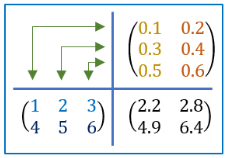
\includegraphics[width=0.8\linewidth]{images/matrixmultiplikation.png}
        \end{center}
        \end{minipage}
    \end{formula}


    
    
    \begin{theorem}{Rechenregeln für die Multiplikation von Matrizen}
        \begin{itemize}
            \item Assoziativ-Gesetz: $A\cdot(B\cdot C)=(A\cdot B)\cdot C$
            \item Distributiv-Gesetz: \\
                $A\cdot(B+C)=A\cdot B+A\cdot C$ und $(A+B)\cdot C=A\cdot C+B\cdot C$
            \item Skalar-Koeffizient: $(\lambda\cdot A)\cdot B=\lambda\cdot (A\cdot B)=A\cdot(\lambda\cdot B)$
        \end{itemize}
    \end{theorem}

    \begin{minipage}{0.65\linewidth}
        \begin{definition}{Transponierte Matrix} $A^{m \times n} \rightarrow (A^T)^{n \times m}$
            \begin{itemize}
                \item $A^T$: Spalten und Zeilen vertauscht
                \item $(A^T)_{ij} = A_{ji}$
            \end{itemize}
            \vspace{2mm}
            $${(A\cdot B)}^T = B^T\cdot A^T$$
        \end{definition}
    \end{minipage}
    \begin{minipage}{0.35\linewidth}
        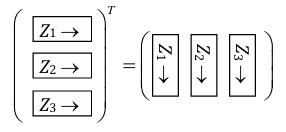
\includegraphics[width=1\linewidth]{images/mat-transpos.png}
    \end{minipage}

    \begin{KR}{Spezielle Matrizen}
        \begin{itemize}
            \item \textbf{Symmetrische Matrix}: $A^T = A$
            \item \textbf{Einheitsmatrix/Identitätsmatrix}: $E$ bzw. $I$\\ mit $e_{ij} = 1$ für $i = j$ und $e_{ij} = 0$ für $i \neq j$
            \item \textbf{Diagonalmatrix}: $a_{ij} = 0$ für $i \neq j$
            \item \textbf{Dreiecksmatrix}: $a_{ij} = 0$ für $i > j$ (obere Dreiecksmatrix) \\oder $i < j$ (untere Dreiecksmatrix)
        \end{itemize}
    \end{KR}

\raggedcolumns
\columnbreak

\subsubsection*{Lineare Gleichungssysteme (LGS)}
    
        \begin{definition}{Lineares Gleichungssystem (LGS)}
            Ein \textit{lineares Gleichungssystem} ist eine Sammlung von Gleichungen, 
            die linear in den Unbekannten sind. 
            Ein LGS kann in Matrixform $A\cdot\vec{x}=\vec{b}$ dargestellt werden.\\
            \begin{minipage}
                {0.45\linewidth}
                {\small
                $A$: Koeffizientenmatrix\\
                $\vec{x}$: Vektor der Unbekannten\\
                $\vec{b}$: Vektor der Konstanten}
            \end{minipage}
            \begin{minipage}{0.55\linewidth}
                $\begin{psmallmatrix} a_{11} & \cdots & a_{1n} \\ \scalebox{0.5}{\vdots} & \cdots & \scalebox{0.5}{\vdots} \\ a_{m1} & \cdots & a_{mn} \end{psmallmatrix} \cdot \begin{psmallmatrix}
                    x_1 \\ \scalebox{0.5}{\vdots} \\ x_n
                \end{psmallmatrix} = \begin{psmallmatrix}
                    b_1 \\ \scalebox{0.5}{\vdots} \\ b_m
                \end{psmallmatrix}$
            \end{minipage}
        \end{definition}

    
        \begin{theorem}{Rang einer Matrix} $rg(A)$ = Anzahl Zeilen - Anzahl Nullzeilen
            
            $\Rightarrow$ Anzahl linear unabhängiger Zeilen- oder Spaltenvektoren
        \end{theorem}


\begin{concept}{Zeilenstufenform (Gauss)}
    \begin{itemize}
        \item Alle Nullen stehen unterhalb der Diagonalen, Nullzeilen zuunterst
        \item Die erste Zahl $\neq 0$ in jeder Zeile ist eine führende Eins
        \item Führende Einsen, die weiter unten stehen $\rightarrow$ stehen weiter rechts
    \end{itemize}
    \textbf{Reduzierte Zeilenstufenform: (Gauss-Jordan)}\\
    Alle Zahlen links und rechts der führenden Einsen sind Nullen.
\end{concept}
    
    \begin{formula}{Gauss-Jordan-Verfahren}
        \begin{enumerate}
            \item bestimme linkeste Spalte mit Elementen $\neq 0$ (Pivot-Spalte)
            \item oberste Zahl in Pivot-Spalte $= 0$\\ $\rightarrow$ vertausche Zeilen so dass $a_{11} \neq 0$
            \item teile erste Zeile durch $a_{11}$ $\rightarrow$ so erhalten wir führende Eins
            \item Nullen unterhalb führender Eins erzeugen (Zeilenperationen)
        \end{enumerate}
        nächste Schritte: ohne bereits bearbeitete Zeilen Schritte 1-4 wiederholen, bis Matrix Zeilenstufenform hat
    \end{formula}

    \begin{KR}{Zeilenperationen} erlaubt bei LGS (z.B. Gauss-Verfahren)
        \begin{itemize}
            \item Vertauschen von Zeilen
            \item Multiplikation einer Zeile mit einem Skalar
            \item Addition eines Vielfachen einer Zeile zu einer anderen
        \end{itemize}
    \end{KR}

    \begin{theorem}{Lösbarkeit von linearen Gleichungssystemen}

        \begin{minipage}{0.5\linewidth}
            \begin{itemize}
                \item Lösbar: $rg(A) = rg(A|b)$
                \item genau eine Lösung: $rg(A) = n$
            \end{itemize}
        \end{minipage}
        \begin{minipage}{0.5\linewidth}
            \begin{itemize}
                \item unendlich viele Lösungen:\\ $rg(A) < n$
            \end{itemize}
        \end{minipage}
    \end{theorem}

    \begin{KR}{Parameterdarstellung} bei unendlich vielen Lösungen

        \begin{minipage}{0.74\linewidth}
            Führende Unbekannte: Spalte mit führender Eins\\
            Freie Unbekannte: Spalten ohne führende Eins
        \end{minipage}
        \begin{minipage}{0.25\linewidth}
            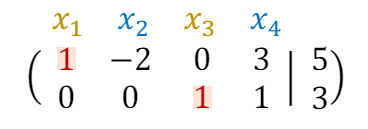
\includegraphics[width=1\linewidth]{images/parameterdarstellung_lgs.png}
        \end{minipage}

        \vspace{1mm}
        
        Auflösung nach der führenden Unbekannten:
        \begin{itemize}
            \item $1 x_1 - 2 x_2 + 0 x_3 + 3 x_4 = 5 \quad x_2 = \lambda \rightarrow x_1 = 5 + 2 \cdot \lambda - 3 \cdot \mu$
            \item $0 x_1 + 0 x_2 + 1 x_3 + 1 x_4 = 3 \quad x_4 = \mu \rightarrow x_3 = 3 - \mu$    
        \end{itemize}
        \vspace*{2mm}
        $$ \vec{x} = \begin{psmallmatrix} x_1 \\ x_2 \\ x_3 \\ x_4 \end{psmallmatrix} 
        = \begin{psmallmatrix} 5 + 2 \lambda - 3 \mu \\ \lambda \\ 3 - \mu \\ \mu \end{psmallmatrix} 
        = \begin{psmallmatrix} 5 \\ 0 \\ 3 \\ 0 \end{psmallmatrix} + \lambda \begin{psmallmatrix} 2 \\ 1 \\ 0 \\ 0 \end{psmallmatrix} + \mu \begin{psmallmatrix} -3 \\ 0 \\ -1 \\ 1 \end{psmallmatrix}$$
    \end{KR}

    \begin{definition}{Homogenes LGS}
        $\vec{b}=\vec{0} \rightarrow A\cdot\vec{x}=\vec{0} \rightarrow rg(A)=rg(A\mid\vec{b})$\\
        nur zwei Möglichkeiten:
            \begin{itemize}
                \item eine Lösung $x_1=x_2=\cdots=x_n=0$, die sog. \textit{triviale Lösung}.
                \item unendlich viele Lösungen
            \end{itemize}
    \end{definition}

    \begin{theorem}{Koeffizientenmatrix{,} Determinante{,} Lösbarkeit des LGS }\\
        Für $n\times n$-Matrix $A$ sind folgende Aussagen äquivalent:
    
        \vspace{1mm}
    
        \begin{minipage}{0.3\linewidth}
            \begin{itemize}
                \item $\det(A)\neq 0$
                \item $rg(A)=n$
                \item $A$ ist invertierbar
            \end{itemize}
        \end{minipage}
        \begin{minipage}{0.7\linewidth}
            \begin{itemize}
                \item Spalten von $A$ sind linear unabhängig.
                \item Zeilen von $A$ sind linear unabhängig.
                \item LGS $A\cdot\vec{x}=\vec{0}$ \\hat eindeutige Lösung $x=A^{-1}\cdot 0=0$
            \end{itemize}
        \end{minipage}
    \end{theorem}


  

\subsubsection*{Quadratische Matrizen}



\begin{formula}{Umformen}
    bestimme die Matrix $X$:
    $A \cdot X + B = 2 \cdot X$

    \vspace{1mm}

    $
    \Rightarrow A \cdot X = 2 \cdot X - B \Rightarrow A \cdot X - 2 \cdot X = -B \Rightarrow (A - 2 \cdot E) \cdot X = -B \\
    \Rightarrow (A - 2 \cdot E) \cdot (A - 2 \cdot E)^{-1} \cdot X = (A - 2 \cdot E)^{-1} \cdot -B \\
    \Rightarrow X = (A - 2 \cdot E)^{-1} \cdot -B
    $
\end{formula}

\paragraph{Inverse}
    \begin{definition}{Inverse einer quadratischen Matrix A} $A^{-1}$ 
        
        $A^{-1}$ existiert, wenn $rg(A) = n$. $A^{-1}$ ist eindeutig bestimmt.

        \vspace{1mm}

        {\small Eine Matrix heisst \textit{invertierbar / regulär}, wenn sie eine Inverse hat. 
        Andernfalls heisst sie \textit{singulär}}
    \end{definition}
  
    \begin{theorem}{Eigenschaften invertierbarer Matrizen}
        \begin{itemize}
            \item $A\cdot A^{-1}=A^{-1}\cdot A=E$
            \item $(A^{-1})^{-1}=A$
            \item ${(A\cdot B)}^{-1}=B^{-1}\cdot A^{-1}$ {\small $\quad$ Die Reihenfolge ist relevant!}\\ $A$ und $B$ invertierbar $\Rightarrow$ $AB$ invertierbar
            \item ${(A^T)^{-1}}={(A^{-1})}^T$ $\quad$ $A$ invertierbar $\Rightarrow$ $A^T$ invertierbar
        \end{itemize}
    \end{theorem}

\begin{theorem}{Inverse einer $2 \times 2$-Matrix} $A = \begin{psmallmatrix} a & b \\ c & d \end{psmallmatrix}$ mit $det(A) = ad - bc$
        $$A^{-1} = \frac{1}{\det(A)} \cdot \begin{pmatrix} d & -b \\ -c & a \end{pmatrix}$$
        NUR Invertierbar falls $ad - bc \neq 0$
\end{theorem}

\begin{KR}{Inverse berechnen} einer quadratischen Matrix $A^{n \times n}$
    $$A \cdot A^{-1} = E \rightarrow \left( A | E \right) \leadsto \text{Zeilenoperationen} \leadsto \left( E | A^{-1}\right)$$
\end{KR}

\begin{example}
    $$
\underbrace{\left(\begin{array}{ccc}
4 & -1 & 0 \\
0 & 2 & 1 \\
3 & -5 & -2
\end{array}\right)}_{A} \cdot \underbrace{\left(\begin{array}{lll}
x_{1} & y_{1} & z_{1} \\
x_{2} & y_{2} & z_{2} \\
x_{3} & y_{3} & z_{3}
\end{array}\right)}_{A^{-1}}=\underbrace{\left(\begin{array}{lll}
1 & 0 & 0 \\
0 & 1 & 0 \\
0 & 0 & 1
\end{array}\right)}_{E}$$
$$ \rightarrow\left(\begin{array}{ccc|ccc}
4 & -1 & 0 & 1 & 0 & 0 \\
0 & 2 & 1 & 0 & 1 & 0 \\
3 & -5 & -2 & 0 & 0 & 1
\end{array}\right)
$$

Zeilenstufenform (linke Seite)

$$ \leadsto 
\left(\begin{array}{ccc|ccc}
1 & -1 / 4 & 0 & 1 / 4 & 0 & 0 \\
0 & 1 & 1 / 2 & 0 & 1 / 2 & 0 \\
0 & 0 & 1 & -6 & 17 & 8
\end{array}\right)
$$

Reduzierte Zeilenstufenform (linke Seite)

$$ \leadsto 
\left(\begin{array}{ccc|ccc}
1 & 0 & 0 & 1 & -2 & -1 \\
0 & 1 & 0 & 3 & -8 & -4 \\
0 & 0 & 1 & -6 & 17 & 8
\end{array}\right) \Rightarrow A^{-1}=\left(\begin{array}{ccc}
1 & -2 & -1 \\
3 & -8 & -4 \\
-6 & 17 & 8
\end{array}\right)
$$
\end{example}



\begin{concept}{LGS mit Inverse lösen}
    $A \cdot \vec{x} = \vec{b}$
    $$A^{-1} \cdot A \cdot \vec{x} = A^{-1} \cdot \vec{b} \rightarrow \vec{x} = A^{-1} \cdot \vec{b}$$
    Beispiel:\\
    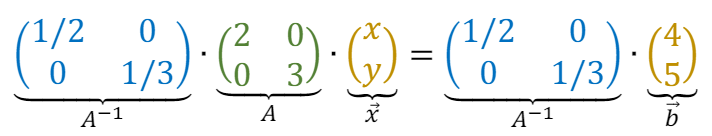
\includegraphics[width=0.7\linewidth]{images/lgs_inverse.png}
\end{concept}




	\raggedcolumns
	

\section{Numerische Lösung linearer Gleichungssysteme}

\begin{KR}{Systematisches Vorgehen bei LGS}
\begin{enumerate}
    \item Eigenschaften der Matrix analysieren:
    \begin{itemize}
        \item Diagonaldominanz prüfen
        \item Konditionszahl berechnen oder abschätzen
        \item Symmetrie erkennen
    \end{itemize}
    
    \item Verfahren auswählen:
    \begin{itemize}
        \item Direkte Verfahren: für kleinere Systeme
        \item Iterative Verfahren: für große, dünnbesetzte Systeme
        \item Spezialverfahren: für symmetrische/bandförmige Matrizen
    \end{itemize}
    
    \item Implementation planen:
    \begin{itemize}
        \item Pivotisierung bei Gauss berücksichtigen
        \item Speicherbedarf beachten
        \item Abbruchkriterien festlegen
    \end{itemize}
\end{enumerate}
\end{KR}

\begin{example2}{Verfahrensauswahl}
Gegeben ist das LGS $Ax = b$ mit:
$$A = \begin{pmatrix} 
4 & -1 & 0 \\
-1 & 4 & -1 \\
0 & -1 & 4
\end{pmatrix}, \quad b = \begin{pmatrix} 1 \\ 0 \\ 1 \end{pmatrix}$$

\paragraph{Analyse:}
\begin{itemize}
    \item Matrix ist symmetrisch
    \item Streng diagonaldominant
    \item Dünnbesetzt (tridiagonal)
\end{itemize}

\paragraph{Verfahrenswahl:}
\begin{itemize}
    \item Gauss: möglich wegen kleiner Dimension
    \item Gauss-Seidel: konvergiert wegen Diagonaldominanz
    \item LR-Zerlegung: effizient wegen Bandstruktur
\end{itemize}
\end{example2}

\begin{concept}{Permutationsmatrix} $P$ ist eine Matrix, die aus der Einheitsmatrix durch Zeilenvertauschungen entsteht. 
    \vspace{1mm}\\
    \begin{minipage}[t]{0.5\textwidth}
        Für die Vertauschung der $i$-ten und $j$-ten Zeile hat $P_k$ die \textbf{Form}:
        \begin{itemize}
            \item $p_{ii} = p_{jj} = 0$ 
            \item $p_{ij} = p_{ji} = 1$
            \item Sonst gleich wie in $E_n$
        \end{itemize}
    \end{minipage}
    \hspace{3mm}
    \begin{minipage}[t]{0.45\textwidth}
        \vspace{1mm}
        \textbf{Wichtige Eigenschaften}:
        \begin{itemize}
            \item $P^{-1} = P^T = P$
            \item Mehrere Vertauschungen:\\ $P = P_l \cdot ... \cdot P_1$
        \end{itemize}
    \end{minipage}
\end{concept}

\begin{example2}{Zeilenvertauschung} für Matrix A mit Permutationsmatrix $P_1$:
    \vspace{1mm}\\
\begin{minipage}[t]{0.5\textwidth}
    $\underbrace{\begin{psmallmatrix}
    1 & 2 & 3\\
    4 & 5 & 6\\
    7 & 8 & 9
    \end{psmallmatrix}}_{A} \cdot 
    \underbrace{\begin{psmallmatrix}
    0 & 0 & 1\\
    0 & 1 & 0\\
    1 & 0 & 0
    \end{psmallmatrix}}_{P_1} =
    \begin{psmallmatrix}
    7 & 8 & 9\\
    4 & 5 & 6\\
    1 & 2 & 3
    \end{psmallmatrix}$
\end{minipage}
\begin{minipage}[t]{0.45\textwidth}
    \vspace{-2mm}
    $\Rightarrow A \cdot P_1$ bewirkt die Vertauschung von Zeile 1 und 3
\end{minipage}
\end{example2}

\vspace{-1mm}
\subsubsection{Pivotisierung}

\begin{concept}{Spaltenpivotisierung}\\
Strategie zur numerischen Stabilisierung des Gauss-Algorithmus durch Auswahl des betragsmäßig größten Elements als Pivotelement.

Vor jedem Eliminationsschritt in Spalte $i$:
\begin{itemize}
    \item Suche $k$ mit $|a_{ki}| = \max\{|a_{ji}| \mid j = i,\ldots,n\}$
    \item Falls $a_{ki} \neq 0$: Vertausche Zeilen $i$ und $k$
    \item Falls $a_{ki} = 0$: Matrix ist singulär
\end{itemize}
\end{concept}

\begin{KR}{Gauss-Algorithmus mit Pivotisierung}\\
\textbf{1. Elimination (Vorwärts)}:
\begin{itemize}
    \item Für $i=1,\ldots,n-1$:
    \begin{itemize}
    \item Finde $k \geq i$ mit $|a_{ki}| = \max\{|a_{ji}| \mid j = i,\ldots,n\}$
    \item Falls $a_{ki} = 0$: Stop (Matrix singulär)
    \item Vertausche Zeilen $i$ und $k$
    \item Für $j=i+1,\ldots,n$:
    \begin{itemize}
    \item $z_j := z_j - \frac{a_{ji}}{a_{ii}}z_i$
    \end{itemize}
    \end{itemize}
\end{itemize}
\vspace{-2mm}
\resizebox{\columnwidth}{!}{
\textbf{2. Rückwärtseinsetzen}:
$x_i = \frac{b_i - \sum_{j=i+1}^n a_{ij}x_j}{a_{ii}}, \quad i=n,n-1,\ldots,1$
}
\end{KR}


\begin{example2}{Gauss mit Pivotisierung}
$A = \begin{psmallmatrix}
0 & 1 & 1\\
2 & 4 & -2\\
0 & 3 & 15
\end{psmallmatrix}, \quad b = \begin{psmallmatrix}
4\\
2\\
36
\end{psmallmatrix}$
\vspace{2mm}\\
\begin{minipage}[t]{0.5\textwidth}
    \textbf{Eliminationsschritte: }
    \vspace{2mm}\\
    $\begin{psmallmatrix}
    2 & 4 & -2 & | & 2\\
    0 & 3 & 15 & | & 36\\
    0 & 1 & 1 & | & 4
    \end{psmallmatrix}
    \Rightarrow
    \begin{psmallmatrix}
    2 & 4 & -2 & | & 2\\
    0 & 3 & 15 & | & 36\\
    0 & 0 & -2 & | & -8
    \end{psmallmatrix}$
\end{minipage}
\begin{minipage}[t]{0.45\textwidth}
    \textbf{Rückwärtseinsetzen: }
    \vspace{1mm}\\
$
\begin{array}{lrl}
    x_3 &= \frac{-8}{-2} = 4\\
    x_2 &= \frac{36 - 15(4)}{3} = 1\\
    x_1 &= \frac{2 - 4(4) + 2}{2} = -6
\end{array}
$
\end{minipage}
\end{example2}

\begin{concept}{Vorteile der Permutationsmatrix}
    \begin{itemize}
        \item Exakte Nachverfolgung aller Zeilenvertauschungen
        \item Einfache Rückführung auf ursprüngliche Reihenfolge durch $P^{-1}$
        \item Kompakte Darstellung mehrerer Vertauschungen
        \item Numerisch stabile Implementierung der Pivotisierung
    \end{itemize}
\end{concept}

\begin{KR}{Zeilenvertauschungen verfolgen}
\begin{enumerate}
    \item Initialisiere $P = I_n$
    \item Für jede Vertauschung von Zeile $i$ und $j$:
    \begin{itemize}
        \item Erstelle $P_k$ durch Vertauschen von Zeilen $i,j$ in $I_n$
        \item Aktualisiere $P = P_k \cdot P$
        \item Wende Vertauschung auf Matrix an: $A := P_kA$
    \end{itemize}
    \item Bei der LR-Zerlegung mit Pivotisierung:
    \begin{itemize}
        \item $PA = LR$ 
        \item Löse $Ly = Pb$ und $Rx = y$
    \end{itemize}
\end{enumerate}
\end{KR}

\begin{KR}{Gauss-Algorithmus mit Pivotisierung}
\begin{enumerate}
    \item Vorbereitung:
    \begin{itemize}
        \item Erweiterte Matrix $(A|b)$ aufstellen
        \item Pivotisierungsstrategie wählen
    \end{itemize}
    
    \item Elimination:
    \begin{itemize}
        \item Für jede Spalte $i$:
        \item Pivotelement in Spalte $i$ bestimmen
        \item Zeilenvertauschung falls nötig
        \item Nullen unterhalb erzeugen
    \end{itemize}
    
    \item Rückwärtseinsetzen:
    $$x_i = \frac{b_i - \sum_{j=i+1}^n a_{ij}x_j}{a_{ii}}, \quad i=n,n-1,\ldots,1$$
    
    \item Kontrolle:
    \begin{itemize}
        \item Residuum $\|Ax-b\|$ berechnen
        \item Pivotisierungsschritte protokollieren
    \end{itemize}
\end{enumerate}
\end{KR}

\begin{example2}{Gauss mit Pivotisierung}
Lösen Sie $Ax = b$ mit:
$$A = \begin{pmatrix} 
1 & 2 & 1 \\
2 & 4 & -1 \\
4 & -2 & 1
\end{pmatrix}, \quad b = \begin{pmatrix} 1 \\ 2 \\ 0 \end{pmatrix}$$

\paragraph{Lösung:}
\begin{enumerate}
    \item Erste Spalte: Pivot $a_{31} = 4$ $\rightarrow$ Z1 $\leftrightarrow $ Z3
    $$\begin{pmatrix} 
    4 & -2 & 1 & | & 0 \\
    2 & 4 & -1 & | & 2 \\
    1 & 2 & 1 & | & 1
    \end{pmatrix}$$
    
    \item Eliminationsschritte:
    $$\begin{pmatrix} 
    4 & -2 & 1 & | & 0 \\
    0 & 5 & -1.5 & | & 2 \\
    0 & 2.5 & 0.75 & | & 1
    \end{pmatrix}$$
    $$\begin{pmatrix} 
    4 & -2 & 1 & | & 0 \\
    0 & 5 & -1.5 & | & 2 \\
    0 & 0 & 1.5 & | & 0.2
    \end{pmatrix}$$
    
    \item Rückwärtseinsetzen:
    \begin{align*}
        x_3 &= 0.2/1.5 = \frac{2}{15} \\
        x_2 &= (2 + 1.5 \cdot \frac{2}{15})/5 = 0.5 \\
        x_1 &= (0 + 2 \cdot 0.5 - 1 \cdot \frac{2}{15})/4 = 0.2
    \end{align*}
\end{enumerate}
\end{example2}

\subsection{Matrix-Zerlegungen}

\begin{definition}{Dreieckszerlegung}
Eine Matrix $A \in \mathbb{R}^{n\times n}$ kann zerlegt werden in:
\vspace{1mm}\\
\begin{minipage}[t]{0.5\textwidth}
    \textbf{Untere Dreiecksmatrix L:}\\
    $l_{ij} = 0$ für $j > i$\\
    Diagonale normiert ($l_{ii}=1$)
\end{minipage}
\hspace{3mm}
\begin{minipage}[t]{0.45\textwidth}
    \textbf{Obere Dreiecksmatrix R:}\\
    $r_{ij} = 0$ für $i > j$\\
    Diagonalelemente $\neq 0$
\end{minipage}
\end{definition}


\subsubsection{LR-Zerlegung}

\begin{theorem}{LR-Zerlegung}\\
Jede reguläre Matrix $A$, für die der Gauss-Algorithmus ohne Zeilenvertauschungen durchführbar ist, lässt sich zerlegen in:
$A = LR$
wobei $L$ eine normierte untere und $R$ eine obere Dreiecksmatrix ist.
\end{theorem}

\begin{KR}{Berechnung der LR-Zerlegung}\\
So berechnen Sie die LR-Zerlegung:
\begin{enumerate}
    \item Führen Sie Gauss-Elimination durch
    \item $R$ ist die resultierende obere Dreiecksmatrix
    \item Die Eliminationsfaktoren $-\frac{a_{ji}}{a_{ii}}$ bilden $L$
    \item Lösen Sie dann nacheinander:
        \begin{itemize}
            \item $Ly = b$ (Vorwärtseinsetzen)
            \item $Rx = y$ (Rückwärtseinsetzen)
        \end{itemize}
\end{enumerate}
\end{KR}

\begin{example2}[breakable]{LR-Zerlegung}
    %TODO: check if this is correct and/or relevant - either correct or replace with better example
$A = \begin{psmallmatrix}
-1 & 1 & 1\\
1 & -3 & -2\\
5 & 1 & 4
\end{psmallmatrix}, \quad b = \begin{psmallmatrix}
0\\
5\\
3
\end{psmallmatrix}$

\paragraph{Schritt 1: Erste Spalte}
Max. Element in 1. Spalte: $|a_{31}| = 5$, also Z1 und Z3 tauschen:
$$P_1 = \begin{psmallmatrix}
0 & 0 & 1\\
0 & 1 & 0\\
1 & 0 & 0
\end{psmallmatrix}, \quad A^{(1)} = \begin{psmallmatrix}
5 & 1 & 4\\
1 & -3 & -2\\
-1 & 1 & 1
\end{psmallmatrix}$$
Berechne Eliminationsfaktoren:
$l_{21} = \frac{1}{5}, \quad l_{31} = -\frac{1}{5}$
\vspace{2mm}\\
Nach Elimination:
$A^{(2)} = \begin{psmallmatrix}
5 & 1 & 4\\
0 & -3.2 & -2.8\\
0 & 1.2 & 1.8
\end{psmallmatrix}$

\paragraph{Schritt 2: Zweite Spalte}
Max. Element in 2. Spalte unter Diagonale: $|-3.2| > |1.2|$, \\ keine Vertauschung nötig.
\vspace{2mm}\\
Berechne Eliminationsfaktor:
$l_{32} = \frac{1.2}{-3.2} = -\frac{3}{8}$
\vspace{2mm}\\
Nach Elimination:
$R = \begin{psmallmatrix}
5 & 1 & 4\\
0 & -3.2 & -2.8\\
0 & 0 & 0.75
\end{psmallmatrix}$

\paragraph{Endergebnis}
Die LR-Zerlegung mit $PA = LR$ ist:
\vspace{2mm}\\
$P = P_1 = \begin{psmallmatrix}
0 & 0 & 1\\
0 & 1 & 0\\
1 & 0 & 0
\end{psmallmatrix}$, 
$L = \begin{psmallmatrix}
1 & 0 & 0\\
\frac{1}{5} & 1 & 0\\
-\frac{1}{5} & -\frac{3}{8} & 1
\end{psmallmatrix}, 
R = \begin{psmallmatrix}
5 & 1 & 4\\
0 & -3.2 & -2.8\\
0 & 0 & 0.75
\end{psmallmatrix}$

\paragraph{Lösung des Systems}
\begin{enumerate}
    \item $Pb = \begin{psmallmatrix} 3\\ 5\\ 0 \end{psmallmatrix}$
    \item Löse $Ly = Pb$ durch Vorwärtseinsetzen:
    $y = \begin{psmallmatrix} 3\\ 4.4\\ 2.25 \end{psmallmatrix}$
    \item Löse $Rx = y$ durch Rückwärtseinsetzen:
    $x = \begin{psmallmatrix} -1\\ -4\\ 3 \end{psmallmatrix}$
\end{enumerate}

\paragraph{Probe}
$$Ax = \begin{psmallmatrix}
-1 & 1 & 1\\
1 & -3 & -2\\
5 & 1 & 4
\end{psmallmatrix} \begin{psmallmatrix} -1\\ -4\\ 3 \end{psmallmatrix} = \begin{psmallmatrix} 0\\ 5\\ 3 \end{psmallmatrix} = b$$
\end{example2}

\begin{KR}{LR-Zerlegung durchführen}
\begin{enumerate}
    \item Zerlegung bestimmen:
    \begin{itemize}
        \item Gauss-Schritte durchführen
        \item Eliminationsfaktoren in $L$ speichern
        \item Resultierende Dreiecksmatrix ist $R$
    \end{itemize}
    
    \item System lösen:
    \begin{itemize}
        \item Vorwärtseinsetzen: $Ly = b$
        \item Rückwärtseinsetzen: $Rx = y$
    \end{itemize}
    
    \item Bei Pivotisierung:
    \begin{itemize}
        \item Permutationsmatrix $P$ erstellen
        \item $PA = LR$ speichern
        \item $Ly = Pb$ lösen
    \end{itemize}
\end{enumerate}
\end{KR}

\begin{example2}{LR-Zerlegung}
Bestimmen Sie die LR-Zerlegung von:
$$A = \begin{pmatrix}
2 & 1 & 1 \\
4 & -2 & -1 \\
-2 & 3 & -1
\end{pmatrix}$$

\paragraph{Lösung:}
\begin{enumerate}
    \item Eliminationsfaktoren:
    \begin{itemize}
        \item $l_{21} = 4/2 = 2$
        \item $l_{31} = -2/2 = -1$
        \item $l_{32} = 1/(-4) = -0.25$
    \end{itemize}
    
    \item Zerlegung:
    $$L = \begin{pmatrix}
    1 & 0 & 0 \\
    2 & 1 & 0 \\
    -1 & -0.25 & 1
    \end{pmatrix}$$
    $$R = \begin{pmatrix}
    2 & 1 & 1 \\
    0 & -4 & -3 \\
    0 & 0 & -0.25
    \end{pmatrix}$$
\end{enumerate}
\end{example2}

\columnbreak

\subsubsection{QR-Zerlegung}

\begin{concept}{QR-Zerlegung}\\
Eine orthogonale Matrix $Q \in \mathbb{R}^{n\times n}$ erfüllt: $Q^T Q = QQ^T = I_n$
\vspace{1mm}\\
Die QR-Zerlegung einer Matrix $A$ ist: $A = QR$
\vspace{1mm}\\
wobei $Q$ orthogonal und $R$ eine obere Dreiecksmatrix ist.
\end{concept}

\begin{definition}{Householder-Transformation}\\
Eine Householder-Matrix hat die Form:
$H = I_n - 2uu^T$

mit $u \in \mathbb{R}^n$, $\|u\| = 1$. Es gilt:
\begin{itemize}
    \item $H$ ist orthogonal ($H^T = H^{-1}$) und symmetrisch ($H^T = H$)
    \item $H^2 = I_n$
\end{itemize}
\end{definition}

\begin{KR}{QR-Zerlegung mit Householder}
\begin{enumerate}
    \item Initialisierung: $R := A$, $Q := I_n$
    \item Für $i = 1,\ldots,n-1$:
        \begin{itemize}
            \item Bilde Vektor $v_i$ aus i-ter Spalte von $R$ ab Position $i$
            \item $w_i := v_i + \text{sign}(v_{i1})\|v_i\|e_1$
            \item $u_i := w_i/\|w_i\|$
            \item $H_i := I_{n-i+1} - 2u_iu_i^T$
            \item Erweitere $H_i$ zu $Q_i$ durch $I_{i-1}$ links oben
            \item $R := Q_iR$ und $Q := QQ_i^T$
        \end{itemize}
\end{enumerate}
\end{KR}

\begin{example2}[breakable]{QR-Zerlegung mit Householder}
    %TODO: check if this is correct and/or relevant - either correct or replace with better example
$A = \begin{psmallmatrix}
2 & 5 & -1\\
-1 & -4 & 2\\
0 & 2 & 1
\end{psmallmatrix}$

\paragraph{Schritt 1: Erste Spalte}
Erste Spalte $a_1$ und Einheitsvektor $e_1$:
$a_1 = \begin{psmallmatrix} 2\\ -1\\ 0 \end{psmallmatrix}, \quad e_1 = \begin{psmallmatrix} 1\\ 0\\ 0 \end{psmallmatrix}$

Householder-Vektor für erste Spalte:
\vspace{1mm}
\begin{enumerate}
    \item Berechne Norm: $|a_1| = \sqrt{2^2 + (-1)^2 + 0^2} = \sqrt{5}$
    \vspace{1mm}
    \item Bestimme Vorzeichen: $\text{sign}(a_{11}) = \text{sign}(2) = 1$
         \begin{itemize}
              \item Wähle positives Vorzeichen, da erstes Element positiv
              \item Dies maximiert die erste Komponente von $v_1$
              \item Verhindert Auslöschung bei der Subtraktion
         \end{itemize}
         \vspace{1mm}
    \item $v_1 = a_1 + \text{sign}(a_{11})|a_1|e_1 = \begin{psmallmatrix} 2\\ -1\\ 0 \end{psmallmatrix} + \sqrt{5}\begin{psmallmatrix} 1\\ 0\\ 0 \end{psmallmatrix} = \begin{psmallmatrix} 2 + \sqrt{5}\\ -1\\ 0 \end{psmallmatrix}$
    \vspace{1mm}
    \item Normiere $v_1$: $|v_1| = \sqrt{(2 + \sqrt{5})^2 + 1} \Rightarrow
            u_1 = \frac{v_1}{|v_1|} = \begin{psmallmatrix} 0.91\\ -0.41\\ 0 \end{psmallmatrix}$
\end{enumerate}
\vspace{1mm}
Householder-Matrix berechnen:
$H_1 = I - 2u_1u_1^T = \begin{psmallmatrix} 
-0.67 & -0.75 & 0\\
-0.75 & 0.67 & 0\\
0 & 0 & 1
\end{psmallmatrix}$
A nach 1. Transformation:
$A^{(1)} = H_1A = \begin{psmallmatrix}
-\sqrt{5} & -6.71 & 0.45\\
0 & -0.89 & 1.79\\
0 & 2.00 & 1.00
\end{psmallmatrix}$
\paragraph{Schritt 2: Zweite Spalte}
Untermatrix für zweite Transformation:
$A_2 = \begin{psmallmatrix} -0.89 & 1.79\\ 2.00 & 1.00 \end{psmallmatrix}$

Householder-Vektor für zweite Spalte:
\vspace{1mm}
\begin{enumerate}
    \item $|a_2| = \sqrt{(-0.89)^2 + 2^2} = 2.19$
    \vspace{1mm}
    \item $\text{sign}(a_{22}) = \text{sign}(-0.89) = -1$ (da erstes Element negativ)
    \vspace{1mm}
    \item $v_2 = \begin{psmallmatrix} -0.89\\ 2.00 \end{psmallmatrix} - 2.19\begin{psmallmatrix} 1\\ 0 \end{psmallmatrix} = \begin{psmallmatrix} -3.09\\ 2.00 \end{psmallmatrix}$
    \vspace{1mm}
    \item $u_2 = \frac{v_2}{|v_2|} = \begin{psmallmatrix} -0.84\\ 0.54 \end{psmallmatrix}$
\end{enumerate}
\vspace{1mm}
Erweiterte Householder-Matrix: %TODO: nicer formatting!
$Q_2 = \begin{psmallmatrix}
1 & 0 & 0\\
0 & -0.41 & -0.91\\
0 & -0.91 & 0.41
\end{psmallmatrix}$

nach 2. Transformation:
$R = Q_2A^{(1)} = \begin{psmallmatrix}
-\sqrt{5} & -6.71 & 0.45\\
0 & -2.19 & 1.34\\
0 & 0 & -1.79
\end{psmallmatrix}$

\paragraph{Endergebnis}
Die QR-Zerlegung $A = QR$ ist:

$Q = H_1^TQ_2^T = \begin{psmallmatrix}
-0.89 & -0.45 & 0\\
0.45 & -0.89 & 0\\
0 & 0 & 1
\end{psmallmatrix},
R = \begin{psmallmatrix}
-\sqrt{5} & -6.71 & 0.45\\
0 & -2.19 & 1.34\\
0 & 0 & -1.79
\end{psmallmatrix}$

\paragraph{Probe}
\small
\begin{enumerate}
    \item $QR = A$ (bis auf Rundungsfehler)
    \item $Q^TQ = QQ^T = I$ (Orthogonalität)
    \item $R$ ist obere Dreiecksmatrix
\end{enumerate}

\paragraph{Wichtige Beobachtungen}
\small
\begin{itemize}
    \item Vorzeichenwahl bei $v_k$ ist entscheidend für numerische Stabilität
    \item Ein falsches Vorzeichen kann zu Auslöschung führen
    \item Betrag der Diagonalelemente in $R$ = Norm transformierter Spalten
    \item $Q$ ist orthogonal: Spaltenvektoren sind orthonormal
\end{itemize}
\end{example2}




\subsubsection{Fehleranalyse}

\begin{definition}{Matrix- und Vektornormen}\\
Eine Vektornorm $\|\cdot\|$ erfüllt für alle $x,y \in \mathbb{R}^n, \lambda \in \mathbb{R}$:
\begin{itemize}
    \item $\|x\| \geq 0$ und $\|x\| = 0 \Leftrightarrow x = 0$
    \item $\|\lambda x\| = |\lambda| \cdot \|x\|$
    \item $\|x + y\| \leq \|x\| + \|y\|$ (Dreiecksungleichung)
\end{itemize}
\end{definition}

\begin{concept}{Wichtige Normen}

\textbf{1-Norm:}
        $\|x\|_1 = \sum_{i=1}^n |x_i|,
        \|A\|_1 = \max_j \sum_{i=1}^n |a_{ij}|$

\textbf{2-Norm:}
        $\|x\|_2 = \sqrt{\sum_{i=1}^n x_i^2}, 
        \|A\|_2 = \sqrt{\rho(A^TA)}$

$\infty$\textbf{-Norm:}
        $\|x\|_\infty = \max_i |x_i|, 
        \|A\|_\infty = \max_i \sum_{j=1}^n |a_{ij}|$
\end{concept}

\begin{theorem}{Fehlerabschätzung für LGS}\\
Sei $\|\cdot\|$ eine Norm, $A \in \mathbb{R}^{n\times n}$ regulär und $Ax = b$, $A\tilde{x} = \tilde{b}$
\vspace{1mm}\\
\begin{minipage}[t]{0.47\textwidth}
    \textbf{Absoluter Fehler:}
    \vspace{-5mm}\\
    \begin{center}
        $\|x - \tilde{x}\| \leq \|A^{-1}\| \cdot \|b - \tilde{b}\|$
    \end{center}
\end{minipage}
\hspace{2mm}
\begin{minipage}[t]{0.47\textwidth}
    \textbf{Relativer Fehler:}
    \vspace{-5mm}\\
    \begin{center}
        $\frac{\|x - \tilde{x}\|}{\|x\|} \leq \text{cond}(A) \cdot \frac{\|b - \tilde{b}\|}{\|b\|}$
    \end{center}
\end{minipage}
\vspace{1mm}\\
Mit der Konditionszahl $\text{cond}(A) = \|A\| \cdot \|A^{-1}\|$
\end{theorem}

\begin{concept}{Konditionierung}\\
Die Konditionszahl beschreibt die numerische Stabilität eines LGS:
\begin{itemize}
    \item $\text{cond}(A) \approx 1$: gut konditioniert
    \item $\text{cond}(A) \gg 1$: schlecht konditioniert
    \item $\text{cond}(A) \to \infty$: singulär
\end{itemize}
\end{concept}

\begin{example2}{Konditionierung}
$A = \begin{psmallmatrix}
1 & 1\\
1 & 1.01
\end{psmallmatrix}, b = \begin{psmallmatrix}
2\\
2.01
\end{psmallmatrix}$\\
Konditionszahl:
$\text{cond}(A) = \|A\| \cdot \|A^{-1}\| \approx 400$
\paragraph{Fehlerabschätzung}
$\text{Absoluter Fehler: }\|x - \tilde{x}\| \leq 400 \cdot 0.01 = 4$ \\
$\text{Relativer Fehler: }\frac{\|x - \tilde{x}\|}{\|x\|} \leq 400 \cdot \frac{0.01}{2} = 2$
\end{example2}

\begin{KR}{Vergleich Lösungsverfahren}
$A = \begin{psmallmatrix}
1 & 2 & 0\\
2 & 1 & 2\\
0 & 2 & 1
\end{psmallmatrix}, \quad b = \begin{psmallmatrix}
1\\
2\\
3
\end{psmallmatrix}$

\small
\begin{itemize}
    \item Matrix ist symmetrisch und nicht streng diagonaldominant
    \item $\text{cond}_\infty(A) \approx 12.5$
\end{itemize}
\begin{center}
\begin{tabular}{l|ccc}
Verfahren & Iterationen & Residuum & Zeit\\
\hline
LR mit Pivot & 1 & $2.2\cdot10^{-16}$ & 1.0\\
QR & 1 & $2.2\cdot10^{-16}$ & 2.3\\
Jacobi & 12 & $1.0\cdot10^{-6}$ & 1.8\\
Gauss-Seidel & 7 & $1.0\cdot10^{-6}$ & 1.4\\
\end{tabular}
\end{center}
\vspace{-2mm}
\begin{itemize}
    \item Direkte Verfahren erreichen höhere Genauigkeit
    \item Iterative Verfahren brauchen mehrere Schritte
\end{itemize}
\end{KR}

\columnbreak

\subsubsection{Iterative Verfahren}

\begin{definition}{Zerlegung der Systemmatrix} $A$ zerlegt in: $A = L + D + R$
    \small
\begin{itemize}
    \item $L$: streng untere Dreiecksmatrix
    \item $D$: Diagonalmatrix
    \item $R$: streng obere Dreiecksmatrix
\end{itemize}
\end{definition}

\begin{concept}{Jacobi-Verfahren}
Gesamtschrittverfahren 
\vspace{1mm}\\
Iteration: $x^{(k+1)} = -D^{-1}(L + R)x^{(k)} + D^{-1}b$
\vspace{1mm}\\
Komponentenweise:
$x_i^{(k+1)} = \frac{1}{a_{ii}}\left(b_i - \sum_{j=1,j\neq i}^n a_{ij}x_j^{(k)}\right)$
\end{concept}

\begin{concept}{Gauss-Seidel-Verfahren}
Einzelschrittverfahren 
\vspace{1mm}\\
Iteration: $x^{(k+1)} = -(D+L)^{-1}Rx^{(k)} + (D+L)^{-1}b$
\vspace{1mm}\\
Komponentenweise:\\
$x_i^{(k+1)} = \frac{1}{a_{ii}}\left(b_i - \sum_{j=1}^{i-1} a_{ij}x_j^{(k+1)} - \sum_{j=i+1}^n a_{ij}x_j^{(k)}\right)$
\end{concept}

\begin{KR}{Implementierung von Jacobi- und Gauss-Seidel-Verfahren}
    \paragraph{Vorbereitungsphase}
    \begin{itemize}
        \item Matrix zerlegen in $A = L + D + R$
        \item Diagonaldominanz prüfen: $|a_{ii}| > \sum_{j\neq i} |a_{ij}|$ für alle $i$
        \item Sinnvolle Startwerte wählen (z.B. $x^{(0)}=0$ oder $x^{(0)}=b$)
        \item Toleranz $\epsilon$ und max. Iterationszahl $n_{max}$ festlegen
    \end{itemize}

    \paragraph{Verfahren durchführen}
    \begin{itemize}
        \item \textbf{Jacobi}: Komponentenweise parallel berechnen 
        \item \textbf{Gauss-Seidel}: Komponentenweise sequentiell berechnen 
    \end{itemize}

    \paragraph{Konvergenzprüfung}
    \begin{itemize}
        \item Absolute Änderung: $\|x^{(k+1)} - x^{(k)}\| < \epsilon$
        \item Relatives Residuum: $\frac{\|Ax^{(k)} - b\|}{\|b\|} < \epsilon$
        \item Maximale Iterationszahl: $k < n_{max}$
    \end{itemize}

    \paragraph{A-priori Fehlerabschätzung}
    \begin{itemize}
        \item Spektralradius $\rho$ der Iterationsmatrix bestimmen
        \item Benötigte Iterationen $n$ für Genauigkeit $\epsilon$:\\
        $n \geq \frac{\ln(\epsilon(1-\rho)/\|x^{(1)}-x^{(0)}\|)}{\ln(\rho)}$
    \end{itemize}
\end{KR}

\begin{KR}{Iterative Verfahren implementieren}
\begin{enumerate}
    \item Matrix zerlegen:
    \begin{itemize}
        \item $A = L + D + R$ für Jacobi
        \item $A = (L+D) + R$ für Gauss-Seidel
    \end{itemize}
    
    \item Konvergenz prüfen:
    \begin{itemize}
        \item Diagonaldominanz
        \item Spektralradius der Iterationsmatrix
    \end{itemize}
    
    \item Iteration durchführen:
    \begin{itemize}
        \item Jacobi: $x^{(k+1)} = -D^{-1}(L+R)x^{(k)} + D^{-1}b$
        \item Gauss-Seidel: $x^{(k+1)} = -(D+L)^{-1}Rx^{(k)} + (D+L)^{-1}b$
    \end{itemize}
    
    \item Abbruchkriterien:
    \begin{itemize}
        \item Residuum: $\|Ax^{(k)}-b\| < \epsilon$
        \item Änderung: $\|x^{(k+1)}-x^{(k)}\| < \epsilon$
        \item Maximale Iterationen
    \end{itemize}
\end{enumerate}
\end{KR}

\begin{example2}{Jacobi vs Gauss-Seidel}
Gegeben sei das System:
$$\begin{pmatrix}
4 & -1 & 0 \\
-1 & 4 & -1 \\
0 & -1 & 4
\end{pmatrix} x = \begin{pmatrix}
1 \\
0 \\
1
\end{pmatrix}$$

\paragraph{Vergleich nach 4 Iterationen:}
\begin{center}
\begin{tabular}{c|cc}
k & Jacobi & Gauss-Seidel \\\hline
1 & 0.250 & 0.250 \\
2 & 0.281 & 0.297 \\
3 & 0.295 & 0.299 \\
4 & 0.298 & 0.300
\end{tabular}
\end{center}

\paragraph{Beobachtungen:}
\begin{itemize}
    \item Gauss-Seidel konvergiert schneller
    \item Beide Verfahren konvergieren monoton
    \item Konvergenz gegen $x_1 = 0.3$
\end{itemize}
\end{example2}

\begin{theorem}{Konvergenzkriterien}
Ein iteratives Verfahren konvergiert, wenn:
\begin{enumerate}
    \item Die Matrix $A$ diagonaldominant ist:\\
    $|a_{ii}| > \sum_{j\neq i} |a_{ij}|$ für alle $i$
    \item Der Spektralradius der Iterationsmatrix kleiner 1 ist:\\
    $\rho(B) < 1$ mit $B$ als jeweilige Iterationsmatrix
\end{enumerate}
\end{theorem}

\begin{example2}{Konvergenzverhalten}
$\begin{psmallmatrix}
4 & 1 & 0\\
1 & 4 & 1\\
0 & 1 & 4
\end{psmallmatrix}
\begin{psmallmatrix}
x_1\\
x_2\\
x_3
\end{psmallmatrix} =
\begin{psmallmatrix}
1\\
2\\
3
\end{psmallmatrix}$
\vspace{1mm}\\
\small
Die Matrix ist diagonaldominant:
$|a_{ii}| = 4 > 1 = \sum_{j\neq i} |a_{ij}|$
\vspace{1mm}\\
\begin{tabular}{c|cc|cc}
k & \multicolumn{2}{c|}{Residuum} & \multicolumn{2}{c}{Rel. Fehler}\\
& Jacobi & G-S & Jacobi & G-S\\
\hline
0 & 3.74 & 3.74 & - & -\\
1 & 0.94 & 0.47 & 0.935 & 0.468\\
2 & 0.23 & 0.06 & 0.246 & 0.125\\
3 & 0.06 & 0.01 & 0.065 & 0.017\\
4 & 0.01 & 0.001 & 0.016 & 0.002
\end{tabular}

\paragraph{Beobachtungen:}
\begin{itemize}
    \item Gauss-Seidel konvergiert etwa doppelt so schnell wie Jacobi
    \item Das Residuum fällt linear (geometrische Folge)
    \item Die Konvergenz ist gleichmäßig (keine Oszillationen)
\end{itemize}
\end{example2}

\subsection{Aufwandsabschätzung}

\begin{concept}{Rechenaufwand}
Anzahl benötigter Gleitkommaoperationen für n×n Systeme:
\begin{itemize}
    \item Gauss-Elimination: $\frac{2}{3}n^3 + \frac{3}{2}n^2 - \frac{13}{6}n$
    \item LR-Zerlegung: $\frac{2}{3}n^3 + \frac{7}{2}n^2 - \frac{13}{6}n$
    \item QR-Zerlegung: $\frac{5}{3}n^3 + 4n^2 + \frac{7}{3}n - 7$
    \item Cramer'sche Regel: $n(n+1)! - 1$ (nicht praktikabel)
\end{itemize}
\end{concept}

\begin{KR}{Aufwand für n×n Systeme abschätzen}
\begin{enumerate}
    \item Hauptterm identifizieren:
    \begin{itemize}
        \item Kubische Terme dominieren für große n
        \item Niedrigere Terme vernachlässigbar
    \end{itemize}
    
    \item Ordnung bestimmen:
    \begin{itemize}
        \item Gauss/LR: $\mathcal{O}(n^3)$
        \item QR: $\mathcal{O}(n^3)$ aber höherer Vorfaktor
        \item Iterative Verfahren: $\mathcal{O}(n^2)$ pro Iteration
    \end{itemize}
    
    \item Speicherbedarf berücksichtigen:
    \begin{itemize}
        \item Direkte Verfahren: $\mathcal{O}(n^2)$
        \item Iterative Verfahren: $\mathcal{O}(n)$ für dünnbesetzte Matrizen
    \end{itemize}
\end{enumerate}
\end{KR}

\begin{example2}{Rechenzeit-Vergleich}
System mit $n=1000$ auf einem 100 GFLOPS Rechner:
\begin{center}
\begin{tabular}{l|cc}
Verfahren & Operationen & Zeit \\
\hline
Gauss & $0.67\cdot10^9$ & 6.7 ms \\
LR & $0.67\cdot10^9$ & 6.7 ms \\
QR & $1.67\cdot10^9$ & 16.7 ms \\
Cramer & $>10^{2567}$ & >Jahre
\end{tabular}
\end{center}
\end{example2}

\subsection{Spezialfälle}

\begin{concept}{Bandmatrizen}
Matrizen mit $a_{ij}=0$ für $|i-j|>m$ (Bandbreite $2m+1$)
\begin{itemize}
    \item Speicheraufwand: $\mathcal{O}(mn)$ statt $\mathcal{O}(n^2)$
    \item Rechenaufwand: $\mathcal{O}(mn^2)$ statt $\mathcal{O}(n^3)$
    \item Häufig bei FEM/Differentialgleichungen
\end{itemize}
\end{concept}

\begin{KR}{Bandmatrizen effizient lösen}
\begin{enumerate}
    \item Speicherformat wählen:
    \begin{itemize}
        \item Nur Diagonalen speichern
        \item Komprimierte Speicherung
        \item Spezielle Datenstrukturen
    \end{itemize}
    
    \item Algorithmen anpassen:
    \begin{itemize}
        \item Nullen außerhalb des Bandes ignorieren
        \item Pivotisierung nur innerhalb Band
        \item Bandstruktur erhalten
    \end{itemize}
    
    \item Effizienz prüfen:
    \begin{itemize}
        \item Bandbreite vs. Systemgröße
        \item Direktes vs. iteratives Verfahren
        \item Speicherverbrauch kontrollieren
    \end{itemize}
\end{enumerate}
\end{KR}

\begin{example2}{Tridiagonales System}
Bandmatrix mit $m=1$ (Bandbreite 3):
$$\begin{pmatrix}
b_1 & c_1 & 0 & 0 \\
a_2 & b_2 & c_2 & 0 \\
0 & a_3 & b_3 & c_3 \\
0 & 0 & a_4 & b_4
\end{pmatrix}
\begin{pmatrix}
x_1 \\ x_2 \\ x_3 \\ x_4
\end{pmatrix} = 
\begin{pmatrix}
d_1 \\ d_2 \\ d_3 \\ d_4
\end{pmatrix}$$

\paragraph{Effizienter Thomas-Algorithmus:}
\begin{enumerate}
    \item Vorwärtselimination:
    \begin{align*}
        c'_1 &= c_1/b_1, \quad d'_1 = d_1/b_1 \\
        b'_i &= b_i - a_ic'_{i-1} \\
        c'_i &= c_i/b'_i \\
        d'_i &= (d_i - a_id'_{i-1})/b'_i
    \end{align*}
    
    \item Rückwärtssubstitution:
    \begin{align*}
        x_n &= d'_n \\
        x_i &= d'_i - c'_ix_{i+1}
    \end{align*}
\end{enumerate}

\paragraph{Komplexität:}
\begin{itemize}
    \item Speicher: $\mathcal{O}(n)$ statt $\mathcal{O}(n^2)$
    \item Rechenzeit: $\mathcal{O}(n)$ statt $\mathcal{O}(n^3)$
\end{itemize}
\end{example2}













	\raggedcolumns
	

\subsection{Komplexe Zahlen}

\begin{examplecode}{Komplexe Zahlen in Python}
\begin{lstlisting}[language=Python, style=basesmol]
def complex_operations(z1, z2):
    """Grundlegende Operationen mit komplexen Zahlen."""
    # Basisfunktionen
    def to_polar(z):
        r = (z.real**2 + z.imag**2)**0.5
        phi = math.atan2(z.imag, z.real)
        return r, phi
    
    def from_polar(r, phi):
        return r * (math.cos(phi) + 1j*math.sin(phi))
    
    try:
        # Addition und Subtraktion
        z_add = z1 + z2
        z_sub = z1 - z2
        
        # Multiplikation und Division
        z_mul = z1 * z2
        z_div = z1 / z2 if z2 != 0 else None
        
        # Polarform
        r1, phi1 = to_polar(z1)
        r2, phi2 = to_polar(z2)
        
        # Exponentialform
        z1_exp = from_polar(r1, phi1)
        z2_exp = from_polar(r2, phi2)
        
        return {
            'addition': z_add,
            'subtraktion': z_sub,
            'multiplikation': z_mul,
            'division': z_div,
            'polar_z1': (r1, phi1),
            'polar_z2': (r2, phi2)
        }
        
    except Exception as e:
        print(f"Fehler bei Berechnung: {e}")
        return None

# Beispiel
z1 = 3 - 11j
z2 = 2 + 5j
results = complex_operations(z1, z2)
\end{lstlisting}
\end{examplecode}

\columnbreak

\section{Komplexe Zahlen}

\begin{lemma}{Fundamentalsatz der Algebra}\\
Eine algebraische Gleichung n-ten Grades mit komplexen Koeffizienten:
$$a_nz^n + a_{n-1}z^{n-1} + \cdots + a_1z + a_0 = 0$$
besitzt in $\mathbb{C}$ genau n Lösungen (mit Vielfachheiten gezählt).
\end{lemma}

\begin{concept}{Komplexe Zahlen}\\
Die Menge der komplexen Zahlen $\mathbb{C}$ erweitert die reellen Zahlen $\mathbb{R}$ durch Einführung der imaginären Einheit $i$ mit der Eigenschaft:
$$i^2 = -1$$

Eine komplexe Zahl $z$ ist ein geordnetes Paar $(x,y)$ mit $x,y \in \mathbb{R}$:
$$z = x + iy$$

Die Menge aller komplexen Zahlen ist definiert als:
$$\mathbb{C} = \{z \mid z = x + iy \text{ mit } x,y \in \mathbb{R}\}$$
\end{concept}

\begin{definition}{Bestandteile komplexer Zahlen}\\
\begin{minipage}[t]{0.6\textwidth}
    \vspace{-7mm}
    \textbf{Realteil:} $\operatorname{Re}(z) = x$\\
    \textbf{Imaginärteil:} $\operatorname{Im}(z) = y$\\
    \textbf{Betrag:} $|z| = \sqrt{x^2 + y^2} = \sqrt{z \cdot z^*}$\\
    \textbf{Konjugation:} $\overline{z} = x - iy$
\end{minipage}
\begin{minipage}{0.35\textwidth}
    \vspace{-3mm}
    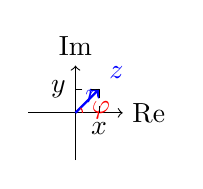
\begin{tikzpicture}[scale=0.3]
        % Coordinate axes
        \draw[->] (-2,0) -- (2,0) node[right] {Re};
        \draw[->] (0,-2) -- (0,2) node[above] {Im};
        
        % Example point and vector
        \draw[thick,blue,->] (0,0) -- (1,1) node[above right] {$z$};
        
        % Angle and labels
        \draw[red] (0.3,0) arc (0:45:0.3) node[midway,right] {$\varphi$};
        
        % Components
        \draw[dashed] (1,1) -- (1,0) node[below] {$x$};
        \draw[dashed] (1,1) -- (0,1) node[left] {$y$};
        
        % Radius
        \node[blue] at (0.7,0.7) {$r$};
    \end{tikzpicture}
\end{minipage}
\end{definition}


\begin{concept}{Darstellungsformen}
\begin{itemize}
    \item Normalform: $z = x + iy$
    \item Trigonometrische Form: $z = r(\cos\varphi + i\sin\varphi)$
    \item Exponentialform: $z = re^{i\varphi}$
\end{itemize}
\end{concept}

\begin{KR}{Umrechnung zwischen Darstellungsformen komplexer Zahlen}
\paragraph{Von Normalform in trigonometrische Form/Exponentialform}
\begin{enumerate}
   \item Berechne Betrag $r = \sqrt{x^2 + y^2}$
   \item Berechne Winkel mit einer der Formeln: 
   \begin{itemize}
       \item $\varphi = \arctan(\frac{y}{x})$ falls $x > 0$
       \item $\varphi = \arctan(\frac{y}{x}) + \pi$ falls $x < 0$
       \item $\varphi = \frac{\pi}{2}$ falls $x = 0, y > 0$
       \item $\varphi = -\frac{\pi}{2}$ falls $x = 0, y < 0$
       \item $\varphi$ unbestimmt falls $x = y = 0$
   \end{itemize}
   \item Trigonometrische Form: $z = r(\cos\varphi + i\sin\varphi)$
   \item Exponentialform: $z = re^{i\varphi}$
\end{enumerate}

\paragraph{Von trigonometrischer Form in Normalform}
\begin{enumerate}
   \item Realteil: $x = r\cos\varphi$
   \item Imaginärteil: $y = r\sin\varphi$
   \item Normalform: $z = x + iy$
\end{enumerate}

\paragraph{Von Exponentialform in Normalform/trigonometrische Form}
\begin{enumerate}
   \item Trigonometrische Form durch Euler-Formel:\\
   $re^{i\varphi} = r(\cos\varphi + i\sin\varphi)$
   \item Dann wie oben in Normalform umrechnen
\end{enumerate}

\paragraph{Wichtige Hinweise:}
\begin{itemize}
   \item Achten Sie auf das korrekte Quadranten beim Winkel
   \item Winkelfunktionen im Bogenmaß verwenden
   \item Bei Umrechnung in Normalform Euler-Formel nutzen
   \item Vorzeichen bei Exponentialform beachten
\end{itemize}
\end{KR}

\begin{theorem}{Rechenoperationen mit komplexen Zahlen}\\
Für $z_1 = x_1 + iy_1$ und $z_2 = x_2 + iy_2$ gilt:
\vspace{1mm}\\
\begin{minipage}[t]{0.45\textwidth}
    \textbf{Addition:}\\
    $z_1 + z_2 = (x_1 + x_2) + i(y_1 + y_2)$
\end{minipage}
\hspace{3mm}
\begin{minipage}[t]{0.45\textwidth}
    \textbf{Subtraktion:}\\
    $z_1 - z_2 = (x_1 - x_2) + i(y_1 - y_2)$
\end{minipage}

\begin{minipage}{0.28\textwidth}
    \textbf{Multiplikation:}
\end{minipage}
\begin{minipage}{0.68\textwidth}
    \begin{align*}
        z_1 \cdot z_2 &= (x_1x_2 - y_1y_2) + i(x_1y_2 + x_2y_1)\\
        &= r_1r_2e^{i(\varphi_1 + \varphi_2)} \text{ (in Exponentialform)}
    \end{align*}
\end{minipage}



\textbf{Division:}
\begin{align*}
    \frac{z_1}{z_2} &= \frac{z_1 \cdot z_2^*}{z_2 \cdot z_2^*} = \frac{(x_1x_2 + y_1y_2) + i(y_1x_2 - x_1y_2)}{x_2^2 + y_2^2}\\
    &= \frac{r_1}{r_2}e^{i(\varphi_1 - \varphi_2)} \text{ (in Exponentialform)}
\end{align*}
\end{theorem}

\begin{theorem}{Potenzen und Wurzeln}\\
Für eine komplexe Zahl in Exponentialform $z = re^{i\varphi}$ gilt:
\begin{itemize}
    \item n-te Potenz: $z^n = r^ne^{in\varphi} = r^n(\cos(n\varphi) + i\sin(n\varphi))$
    \item n-te Wurzel: $z_k = \sqrt[n]{r}e^{i\frac{\varphi + 2\pi k}{n}}$, $k = 0,1,\ldots,n-1$
\end{itemize}
\end{theorem}


\section{Eigenwerte und Eigenvektoren}

\begin{definition}{Eigenwerte und Eigenvektoren}\\
Für eine Matrix $A \in \mathbb{R}^{n\times n}$ heißt $\lambda \in \mathbb{C}$ Eigenwert von $A$, wenn es einen Vektor $x \in \mathbb{C}^n \backslash \{0\}$ gibt mit:
\vspace{-2mm}\\
$$Ax = \lambda x$$
Der Vektor $x$ heißt dann Eigenvektor zum Eigenwert $\lambda$.
\end{definition}

\begin{concept}{Bestimmung von Eigenwerten}\\
Ein Skalar $\lambda$ ist genau dann Eigenwert von $A$, wenn gilt:
\vspace{-2mm}\\
$$\det(A - \lambda I_n) = 0$$
Diese Gleichung heißt charakteristische Gleichung. Das zugehörige Polynom
\vspace{-2mm}
$$p(\lambda) = \det(A - \lambda I_n)$$
ist das charakteristische Polynom von $A$.
\end{concept}

\begin{theorem}{Eigenschaften von Eigenwerten}
Für eine Matrix $A \in \mathbb{R}^{n\times n}$ gilt:
$$\det(A) = \prod_{i=1}^n \lambda_i \text{ (Produkt der Eigenwerte)}$$
$$\operatorname{tr}(A) = \sum_{i=1}^n \lambda_i \text{ (Summe der Eigenwerte)}$$
\begin{itemize}
    \item Bei Dreiecksmatrix sind die Diagonalelemente die Eigenwerte
    \item Ist $\lambda$ Eigenwert von $A$, so ist $\frac{1}{\lambda}$ Eigenwert von $A^{-1}$
\end{itemize}
\end{theorem}

\begin{concept}{Vielfachheiten}
Für einen Eigenwert $\lambda$ unterscheidet man:
\begin{itemize}
    \item Algebraische Vielfachheit: \\Vielfachheit als Nullstelle des charakteristischen Polynoms
    \item Geometrische Vielfachheit: \\Dimension des Eigenraums $= n - \operatorname{rg}(A-\lambda I_n)$
\end{itemize}
Die geometrische Vielfachheit ist stets kleiner oder gleich der algebraischen Vielfachheit.
\end{concept}

\begin{KR}{Bestimmung von Eigenwerten und Eigenvektoren}
\paragraph{Vorbereitung}
\begin{itemize}
    \item Matrix $A \in \mathbb{R}^{n \times n}$ aufschreiben
    \item Charakteristische Matrix $(A - \lambda I)$ aufstellen
\end{itemize}

\paragraph{Eigenwerte bestimmen}
\begin{enumerate}
    \item Charakteristisches Polynom aufstellen:
    \begin{itemize}
        \item Bei $2 \times 2$ Matrizen direkt: $\det(A - \lambda I)$
        \item Bei $3 \times 3$ Matrizen: Entwicklung nach einer Zeile/Spalte
        \item Bei größeren Matrizen: Spezielle Eigenschaften nutzen
              (z.B. Dreiecksform, Symmetrie)
    \end{itemize}
    
    \item Polynom vereinfachen und auf Nullform bringen:
    \begin{itemize}
        \item Ausmultiplizieren
        \item Zusammenfassen nach Potenzen von $\lambda$
        \item Form: $p(\lambda) = (-1)^n\lambda^n + a_{n-1}\lambda^{n-1} + \cdots + a_1\lambda + a_0$
    \end{itemize}

    \item Nullstellen bestimmen:
    \begin{itemize}
        \item Bei quadratischer Gleichung: Mitternachtsformel
        \item Bei Grad 3: Substitution oder Cardanische Formeln
        \item Bei höherem Grad: Numerische Verfahren
    \end{itemize}
\end{enumerate}

\paragraph{Eigenvektoren bestimmen}
\begin{enumerate}
    \item Für jeden Eigenwert $\lambda_i$:
    \begin{itemize}
        \item Matrix $(A - \lambda_i I)$ aufstellen
        \item Homogenes LGS $(A - \lambda_i I)x = 0$ lösen
        \item Lösungsvektor normieren falls gewünscht
    \end{itemize}

    \item Bei mehrfachen Eigenwerten:
    \begin{itemize}
        \item Basis des Eigenraums bestimmen
        \item Linear unabhängige Eigenvektoren finden
    \end{itemize}
\end{enumerate}

\paragraph{Kontrolle}
\begin{itemize}
    \item Für jeden Eigenvektor $x_i$ prüfen: $Ax_i = \lambda_i x_i$
    \item Bei $2 \times 2$ Matrix: $\lambda_1 + \lambda_2 = \operatorname{tr}(A)$ und $\lambda_1 \cdot \lambda_2 = \det(A)$
    \item Bei $3 \times 3$ Matrix zusätzlich: $\sum \lambda_i = \operatorname{tr}(A)$ und $\prod \lambda_i = \det(A)$
    \item Bei reellen Matrizen: Komplexe Eigenwerte treten in konjugierten Paaren auf
\end{itemize}

\paragraph{Spezialfälle beachten}
\begin{itemize}
    \item Bei Dreiecksmatrizen: Eigenwerte sind die Diagonalelemente
    \item Bei symmetrischen Matrizen: Alle Eigenwerte sind reell
    \item Bei orthogonalen Matrizen: $|\lambda_i| = 1$ für alle Eigenwerte
    \item Bei nilpotenten Matrizen: Alle Eigenwerte sind 0
\end{itemize}
\end{KR}

\begin{example2}{Eigenwertberechnung}
Gegeben ist die Matrix
$A = \begin{psmallmatrix} 
2 & 1 & 0 \\
1 & 2 & 1 \\
0 & 1 & 2
\end{psmallmatrix}$

1. Charakteristisches Polynom aufstellen:
   $$\det(A - \lambda I) = \begin{vsmallmatrix} 
   2-\lambda & 1 & 0 \\
   1 & 2-\lambda & 1 \\
   0 & 1 & 2-\lambda
   \end{vsmallmatrix}$$
   
2. Entwicklung nach 1. Zeile:
   $$p(\lambda) = (2-\lambda)\begin{vsmallmatrix}
   2-\lambda & 1 \\
   1 & 2-\lambda
   \end{vsmallmatrix} - 1\begin{vsmallmatrix}
   1 & 1 \\
   1 & 2-\lambda
   \end{vsmallmatrix}$$
   
3. Ausrechnen:
   $$p(\lambda) = (2-\lambda)((2-\lambda)^2 - 1) - ((2-\lambda) - 1)
   = -\lambda^3 + 6\lambda^2 - 11\lambda + 6$$
   
4. Nullstellen bestimmen:
   $\lambda_1 = 1, \lambda_2 = 2, \lambda_3 = 3$
\vspace{1mm}\\
5. Eigenvektoren bestimmen für $\lambda_1 = 1$:
   $$(A - I)x = 0 \text{ führt zu } x_1 = \begin{psmallmatrix} 1 \\ -2 \\ 1 \end{psmallmatrix}$$
\end{example2}

\begin{examplecode}{Determinante}
\begin{lstlisting}[language=Python, style=basesmol]
def det_2x2(matrix):
    return matrix[0][0]*matrix[1][1] - matrix[0][1]*matrix[1][0]

def det_3x3(matrix):
    det = 0
    # Entwicklung nach erster Zeile
    for i in range(3):
        minor = []
        for j in range(1,3):
            row = []
            for k in range(3):
                if k != i:
                    row.append(matrix[j][k])
            minor.append(row)
        det += ((-1)**i) * matrix[0][i] * det_2x2(minor)
    return det
\end{lstlisting}
\end{examplecode}

\begin{examplecode}{Charakteristisches Polynom Koeffizienten berechnen}
\begin{lstlisting}[language=Python, style=basesmol]
def char_poly_coeff(matrix):
    n = len(matrix)
    coeffs = [0] * (n+1)
    # Lambda^n Koeffizient
    coeffs[n] = (-1)**n
    # Spur (Lambda^(n-1) Koeffizient)
    trace = sum(matrix[i][i] for i in range(n))
    coeffs[n-1] = (-1)**(n-1) * trace
    # Determinante (konstanter Term)
    coeffs[0] = det_3x3(matrix)
    
    return coeffs

# Beispielmatrix
A = [[2, 1, 0],
     [1, 2, 1],
     [0, 1, 2]]

# Charakteristisches Polynom berechnen
poly = char_poly_coeff(A)
print("Charakteristisches Polynom:")
print(f"p(lambda) = lambda^3 {poly[2]:+}lambda^2 {poly[1]:+}lambda {poly[0]:+}")
\end{lstlisting}
\end{examplecode}

\begin{examplecode}{Eigenvektoren berechnen} \textcolor{pink}{\texttt{use Gauss from previous example}} 
\begin{lstlisting}[language=Python, style=basesmol]
def find_eigenvector(A, eigenvalue):
    n = len(A)
    # A - lambda*I
    A_lambda = [[A[i][j] - (eigenvalue if i==j else 0) 
                for j in range(n)] for i in range(n)]
    
    # Loese (A - lambda*I)x = 0
    b = [0] * n
    return gauss_elimination(A_lambda, b)

# Eigenvektoren fuer lambda = 1,2,3 berechnen
eigenvalues = [1, 2, 3]
for ev in eigenvalues:
    vec = find_eigenvector(A, ev)
    print(f"Eigenvektor fuer lambda={ev}:", vec)
\end{lstlisting}
\end{examplecode}



\subsubsection{Numerische Berechnung von Eigenwerten}

\begin{concept}{Ähnliche Matrizen}\\
Zwei Matrizen $A,B \in \mathbb{R}^{n\times n}$ heißen ähnlich, wenn es eine reguläre Matrix $T$ gibt mit:
$$B = T^{-1}AT$$

Eine Matrix $A$ heißt diagonalisierbar, wenn sie ähnlich zu einer Diagonalmatrix $D$ ist:
$$D = T^{-1}AT$$
\end{concept}

\begin{theorem}{Eigenschaften ähnlicher Matrizen}\\
Für ähnliche Matrizen $A$ und $B = T^{-1}AT$ gilt:
\begin{enumerate}
    \item $A$ und $B$ haben dieselben Eigenwerte mit gleichen algebraischen Vielfachheiten
    \item Ist $x$ Eigenvektor von $B$ zum Eigenwert $\lambda$, so ist $Tx$ Eigenvektor von $A$ zum Eigenwert $\lambda$
    \item Bei Diagonalisierbarkeit:
    \begin{itemize}
        \item Die Diagonalelemente von $D$ sind die Eigenwerte von $A$
        \item Die Spalten von $T$ sind die Eigenvektoren von $A$
    \end{itemize}
\end{enumerate}
\end{theorem}

\begin{definition}{Spektralradius}
Der Spektralradius einer Matrix $A$ ist definiert als:
$$\rho(A) = \max\{|\lambda| \mid \lambda \text{ ist Eigenwert von } A\}$$
Er gibt den Betrag des betragsmäßig größten Eigenwerts an.
\end{definition}

\subsubsection{Von-Mises-Iteration}

\begin{concept}{Von-Mises-Iteration (Vektoriteration)}\\
Für eine diagonalisierbare Matrix $A$ mit Eigenwerten $|\lambda_1| > |\lambda_2| \geq \cdots \geq |\lambda_n|$ konvergiert die Folge:
$$v^{(k+1)} = \frac{Av^{(k)}}{\|Av^{(k)}\|_2}, \quad
\lambda^{(k+1)} = \frac{(v^{(k)})^TAv^{(k)}}{(v^{(k)})^Tv^{(k)}}$$
gegen einen Eigenvektor $v$ zum betragsmäßig größten Eigenwert $\lambda_1$.
\end{concept}

\begin{KR}{Von-Mises-Iteration durchführen}
\begin{enumerate}
    \item Wähle Startvektor $v^{(0)}$ mit $\|v^{(0)}\|_2 = 1$
    \item Für $k = 0,1,2,\ldots$:
    \begin{itemize}
        \item Berechne $w^{(k)} = Av^{(k)}$
        \item Normiere: $v^{(k+1)} = \frac{w^{(k)}}{\|w^{(k)}\|_2}$
        \item Berechne Rayleigh-Quotienten $\lambda^{(k+1)}$
        \item Prüfe Konvergenz
    \end{itemize}
\end{enumerate}
\end{KR}

\begin{example2}{Von-Mises-Iteration}
Berechne größten Eigenwert der Matrix:
\vspace{2mm}\\
$A = \begin{psmallmatrix}
4 & -1 & 1\\
-1 & 3 & -2\\
1 & -2 & 3
\end{psmallmatrix}$, $\quad$
Startvektor: $v^{(0)} = \begin{psmallmatrix}1\\ 0\\ 0\end{psmallmatrix}$

\begin{center}
\begin{tabular}{c|c|c}
k & $v^{(k)}$ & $\lambda^{(k)}$ \\\hline
0 & $(1, 0, 0)^T$ & -\\
1 & $(0.970, -0.213, 0.119)^T$ & 4.000\\
2 & $(0.957, -0.239, 0.164)^T$ & 4.827\\
3 & $(0.953, -0.244, 0.178)^T$ & 4.953\\
4 & $(0.952, -0.245, 0.182)^T$ & 4.989
\end{tabular}
\end{center}

Konvergenz gegen $\lambda_1 \approx 5$ \\ Eigenvektor $v \approx (0.952, -0.245, 0.182)^T$
\end{example2}

\begin{KR}{Von-Mises-Iteration / Vektoriteration}
\paragraph{Voraussetzungen}
\begin{itemize}
    \item Matrix $A \in \mathbb{R}^{n \times n}$ diagonalisierbar
    \item Betragsmäßig größter Eigenwert ist eindeutig: $|\lambda_1| > |\lambda_2| \geq \cdots \geq |\lambda_n|$
\end{itemize}

\paragraph{Algorithmus}
\begin{enumerate}
    \item Startvektor $v^{(0)}$ wählen:
    \begin{itemize}
        \item Zufälligen Vektor oder $(1,\ldots,1)^T$ wählen
        \item Auf Länge 1 normieren: $\|v^{(0)}\|_2 = 1$
    \end{itemize}

    \item Für $k = 0,1,2,\ldots$ bis zur Konvergenz:
    \begin{itemize}
        \item Iterationsvektor berechnen: $w^{(k)} = Av^{(k)}$
        \item Normieren: $v^{(k+1)} = \frac{w^{(k)}}{\|w^{(k)}\|_2}$
        \item Eigenwertapproximation (Rayleigh-Quotient):
              $\lambda^{(k+1)} = \frac{(v^{(k)})^TAv^{(k)}}{(v^{(k)})^Tv^{(k)}}$
    \end{itemize}

    \item Abbruchkriterien prüfen:
    \begin{itemize}
        \item Änderung des Eigenvektors: $\|v^{(k+1)} - v^{(k)}\| < \varepsilon$
        \item Änderung des Eigenwertes: $|\lambda^{(k+1)} - \lambda^{(k)}| < \varepsilon$
        \item Maximale Iterationszahl erreicht
    \end{itemize}
\end{enumerate}

\paragraph{Verifikation}
\begin{itemize}
    \item Prüfen ob $Av^{(k)} \approx \lambda^{(k)}v^{(k)}$
    \item Residuum berechnen: $\|Av^{(k)} - \lambda^{(k)}v^{(k)}\|$
    \item Orthogonalität zu anderen Eigenvektoren prüfen
\end{itemize}
\end{KR}

\begin{example2}{Von-Mises-Iteration}
Gegeben sei die Matrix
$A = \begin{pmatrix} 
4 & -1 & 1 \\
-1 & 3 & -2 \\
1 & -2 & 3
\end{pmatrix}$

Mit Startvektor $v^{(0)} = \frac{1}{\sqrt{3}}(1,1,1)^T$:

\begin{enumerate}
    \item Erste Iteration:
    \begin{itemize}
        \item $w^{(0)} = Av^{(0)} = \frac{1}{\sqrt{3}}(4,0,2)^T$
        \item $v^{(1)} = \frac{w^{(0)}}{\|w^{(0)}\|} = \frac{1}{\sqrt{20}}(4,0,2)^T$
        \item $\lambda^{(1)} = (v^{(0)})^TAv^{(0)} = 3.33$
    \end{itemize}

    \item Zweite Iteration:
    \begin{itemize}
        \item $w^{(1)} = Av^{(1)} = \frac{1}{\sqrt{20}}(18,-2,8)^T$
        \item $v^{(2)} = \frac{w^{(1)}}{\|w^{(1)}\|} = \frac{1}{\sqrt{388}}(18,-2,8)^T$
        \item $\lambda^{(2)} = 5.12$
    \end{itemize}

Konvergenz gegen $\lambda_1 \approx 5.17$ und $v = (0.89, -0.10, 0.39)^T$
\end{enumerate}
\end{example2}

\begin{KR}{QR-Verfahren}
\paragraph{Voraussetzungen}
\begin{itemize}
    \item Matrix $A \in \mathbb{R}^{n \times n}$
    \item Eigenwerte sollten verschiedene Beträge haben für gute Konvergenz
\end{itemize}

\paragraph{Algorithmus}
\begin{enumerate}
    \item Initialisierung:
    \begin{itemize}
        \item $A_0 := A$
        \item $Q_0 := I_n$
    \end{itemize}

    \item Für $k = 0,1,2,\ldots$ bis zur Konvergenz:
    \begin{itemize}
        \item QR-Zerlegung von $A_k$ berechnen: $A_k = Q_kR_k$
        \item Neue Matrix berechnen: $A_{k+1} = R_kQ_k$
        \item Transformationsmatrix aktualisieren: $P_{k+1} = P_kQ_k$
    \end{itemize}

    \item Abbruchkriterien prüfen:
    \begin{itemize}
        \item Subdiagonalelemente nahe Null: $|a_{i+1,i}| < \varepsilon$
        \item Änderung der Diagonalelemente klein
        \item Maximale Iterationszahl erreicht
    \end{itemize}
\end{enumerate}

\paragraph{Auswertung}
\begin{itemize}
    \item Eigenwerte: Diagonalelemente von $A_k$
    \item Eigenvektoren: Spalten der Matrix $P_k$
    \item Bei $2\times2$-Blöcken: Komplexe Eigenwertpaare
\end{itemize}
\end{KR}

\begin{example2}{QR-Verfahren}
Gegeben sei die Matrix
$A = \begin{pmatrix} 
1 & 2 & 0 \\
2 & 1 & 1 \\
0 & 1 & 1
\end{pmatrix}$

\begin{enumerate}
    \item Erste Iteration:
    \begin{itemize}
        \item QR-Zerlegung:
        $Q_1 = \begin{pmatrix} 
        0.45 & 0.89 & 0 \\
        0.89 & -0.45 & 0 \\
        0 & 0 & 1
        \end{pmatrix}$,
        $R_1 = \begin{pmatrix}
        2.24 & 2.24 & 0.45 \\
        0 & -1 & 0.89 \\
        0 & 0 & 1
        \end{pmatrix}$
        \item $A_1 = R_1Q_1 = \begin{pmatrix}
        2.24 & 0.45 & 0.45 \\
        0.45 & 0.38 & 0.89 \\
        0.45 & 0.89 & 1
        \end{pmatrix}$
    \end{itemize}

    \item Nach Konvergenz:
    $A_k \approx \begin{pmatrix}
    3 & * & * \\
    0 & 0 & * \\
    0 & 0 & 0
    \end{pmatrix}$

    Eigenwerte sind also $\lambda_1 = 3, \lambda_2 = 0, \lambda_3 = 0$
\end{enumerate}
\end{example2}

\begin{examplecode}{Von-Mises-Iteration}
\begin{lstlisting}[language=Python, style=basesmol]
def matrix_vector_mult(A, v):
    n = len(A)
    result = [0] * n
    for i in range(n):
        for j in range(n):
            result[i] += A[i][j] * v[j]
    return result

def vector_norm(v):
    return sum(x*x for x in v) ** 0.5

def normalize_vector(v):
    norm = vector_norm(v)
    return [x/norm for x in v]

def power_iteration(A, tol=1e-10, max_iter=100):
    n = len(A)
    # Startvektor
    v = normalize_vector([1] + [0]*(n-1))
    
    for _ in range(max_iter):
        # Matrix-Vektor-Multiplikation
        w = matrix_vector_mult(A, v)
        # Normierung
        v_new = normalize_vector(w)
        
        # Rayleigh-Quotient
        lambda_k = sum(v_new[i] * A[i][j] * v_new[j] 
                      for i in range(n) 
                      for j in range(n))
        
        # Konvergenzpruefung
        if vector_norm([v_new[i]-v[i] for i in range(n)]) < tol:
            return lambda_k, v_new
            
        v = v_new
    return lambda_k, v
\end{lstlisting}
\end{examplecode}

\subsubsection{QR-Verfahren}

\begin{concept}{QR-Verfahren}\\
Das QR-Verfahren transformiert die Matrix $A$ iterativ in eine obere Dreiecksmatrix, deren Diagonalelemente die Eigenwerte sind:
\begin{enumerate}
    \item Initialisierung: $A_0 := A$, $P_0 := I_n$
    \item Für $i = 0,1,2,\ldots$:
    \begin{itemize}
        \item QR-Zerlegung: $A_i = Q_iR_i$
        \item Neue Matrix: $A_{i+1} = R_iQ_i$
        \item Update: $P_{i+1} = P_iQ_i$
    \end{itemize}
\end{enumerate}
\end{concept}

\begin{KR}{QR-Verfahren anwenden}
    %TODO: check if this is correct and/or relevant - either correct or replace with better example
\begin{enumerate}
    \item Matrix $A_0 = A$ vorbereiten
    \item In jedem Schritt $i$:
    \begin{itemize}
        \item QR-Zerlegung mit Householder oder Givens
        \item Neue Matrix durch Multiplikation $R_iQ_i$
        \item Konvergenz prüfen: Subdiagonalelemente $\approx$ 0?
    \end{itemize}
    \item Eigenwerte: Diagonalelemente der Endmatrix
    \item Eigenvektoren: Spalten von $P = P_1P_2\cdots P_k$
\end{enumerate}
\end{KR}

\begin{example2}{QR-Verfahren}
    %TODO: add example
\end{example2}



\begin{example2}{QR-Verfahren}
Matrix:
$$A = \begin{psmallmatrix}
2 & -1 & 1\\
-1 & 3 & 0\\
1 & 0 & 1
\end{psmallmatrix}$$

\paragraph{QR-Iteration:}
\begin{enumerate}
    \item $A_0 = A$
    \item Nach erster Iteration:
    $$A_1 = \begin{psmallmatrix}
    3.21 & -0.83 & 0.62\\
    -0.83 & 2.13 & 0.41\\
    0.62 & 0.41 & 0.66
    \end{psmallmatrix}$$
    \item Nach 5 Iterationen:
    $$A_5 \approx \begin{psmallmatrix}
    4 & 0 & 0\\
    0 & 1 & 0\\
    0 & 0 & 1
    \end{psmallmatrix}$$
\end{enumerate}

Die Diagonalelemente von $A_5$ sind die Eigenwerte: $\lambda_1 = 4, \lambda_2 = 1, \lambda_3 = 1$
\end{example2}

\begin{examplecode}{QR-Verfahren}
\begin{lstlisting}[language=Python, style=basesmol]
def matmul(A, B):
    n = len(A)
    C = [[0.0] * n for _ in range(n)]
    for i in range(n):
        for j in range(n):
            C[i][j] = sum(A[i][k] * B[k][j] 
                     for k in range(n))
    return C

def transpose(A):
    n = len(A)
    return [[A[j][i] for j in range(n)] 
            for i in range(n)]

def householder(x):
    n = len(x)
    # Norm berechnen
    s = sum(x[i]**2 for i in range(1, n))
    v = [0.0] * n
    if s == 0:
        return v
    
    v[0] = x[0]
    norm_x = (x[0]**2 + s)**0.5
    if x[0] <= 0:
        v[0] = x[0] - norm_x
    else:
        v[0] = -s/(x[0] + norm_x)
    
    for i in range(1, n):
        v[i] = x[i]
    
    return normalize_vector(v)

def qr_algorithm(A, tol=1e-10, max_iter=100):
    n = len(A)
    A_k = [row[:] for row in A]  # Kopiere A
    
    for k in range(max_iter):
        # QR-Zerlegung mit Householder
        Q = [[1.0 if i==j else 0.0 
              for j in range(n)] 
              for i in range(n)]
        R = [row[:] for row in A_k]
        
        for j in range(n-1):
            v = householder([R[i][j] 
                 for i in range(j, n)])
            # Householder-Transformation anwenden
            
        # Neue Iteration A_(k+1) = RQ
        A_k = matmul(R, Q)
        
        # Konvergenztest
        if max(abs(A_k[i][j]) 
               for i in range(1, n) 
               for j in range(i)) < tol:
            break
    
    return [A_k[i][i] for i in range(n)]
\end{lstlisting}
\end{examplecode}

\begin{remark2}{Numerische Stabilität}
\begin{itemize}
    \item QR-Verfahren ist numerisch stabiler als Vektoriteration
    \item Findet alle Eigenwerte, nicht nur den größten
    \item Benötigt mehr Rechenaufwand
    \item Konvergiert linear für reelle, quadratisch für komplexe Eigenwerte
\end{itemize}
\end{remark2}

\subsection{Praktische Anwendungen}

\begin{concept}{Anwendungen von Eigenwerten}
\begin{itemize}
    \item Bestimmung von Schwingungsmoden in mechanischen Systemen
    \item Hauptkomponentenanalyse in der Datenanalyse
    \item Stabilität von dynamischen Systemen
    \item PageRank-Algorithmus für Webseitenranking
    \item Bildkompression und Signalverarbeitung
\end{itemize}
\end{concept}

\begin{example2}{PageRank-Algorithmus}
Google-Matrix für ein kleines Webnetzwerk mit 3 Seiten:
$$A = \begin{psmallmatrix}
0 & 1/2 & 1/3\\
1 & 0 & 1/3\\
0 & 1/2 & 1/3
\end{psmallmatrix}$$

Der PageRank entspricht dem Eigenvektor zum Eigenwert 1:
\begin{itemize}
    \item $\lambda = 1$ ist größter Eigenwert
    \item PageRank: $v \approx (0.39, 0.41, 0.20)^T$
    \item Seite 2 hat höchste Relevanz, Seite 3 niedrigste
\end{itemize}
\end{example2}

\begin{KR}{Praktische Eigenwertberechnung}
\begin{enumerate}
    \item Vorverarbeitung der Matrix:
    \begin{itemize}
        \item Auf Symmetrie prüfen
        \item Ggf. auf Hessenberg-Form transformieren
        \item Kondition der Matrix prüfen
    \end{itemize}
    
    \item Wahl des geeigneten Verfahrens:
    \begin{itemize}
        \item Nur größter EW → Von-Mises
        \item Alle EW → QR-Verfahren
        \item Symmetrisch → Symmetrisches QR
        \item Einzelner EW → Inverse Iteration
    \end{itemize}
    
    \item Implementierungsaspekte:
    \begin{itemize}
        \item Konvergenzkriterien definieren
        \item Numerische Stabilität sicherstellen
        \item Abbruchkriterien festlegen
        \item Fehlerbehandlung implementieren
    \end{itemize}
    
    \item Nachbearbeitung:
    \begin{itemize}
        \item Genauigkeit überprüfen
        \item EV auf Länge 1 normieren
        \item Komplexe EW/EV behandeln
        \item Ergebnisse validieren
    \end{itemize}
\end{enumerate}
\end{KR}

\begin{examplecode}{Inverse Iteration}
\begin{lstlisting}[language=Python, style=basesmol]
def inverse_iteration(A, mu, tol=1e-10, max_iter=100):
    n = len(A)
    # Startvektor
    v = [1.0] + [0.0] * (n-1)
    v = normalize_vector(v)
    
    # Matrix (A - mu*I) erstellen
    A_shift = [[A[i][j] if i != j 
                else A[i][j] - mu 
                for j in range(n)] 
              for i in range(n)]
    
    for k in range(max_iter):
        # Loese (A - mu*I)w = v
        w = solve_linear_system(A_shift, v)
        # Normiere Ergebnisvektor
        v_new = normalize_vector(w)
        
        # Konvergenztest
        if vector_norm([v_new[i]-v[i] 
                     for i in range(n)]) < tol:
            # Berechne Rayleigh-Quotienten
            lambda_k = rayleigh_quotient(A, v_new)
            return lambda_k, v_new
            
        v = v_new
    
    raise ValueError("Keine Konvergenz")

def solve_linear_system(A, b):
    # LR-Zerlegung und Rueckwaertseinsetzen
    n = len(A)
    x = gauss_solve(A, b)  # aus LGS Kapitel
    return x
\end{lstlisting}
\end{examplecode}

\begin{example2}{Inverse Iteration}
Matrix mit bekanntem Eigenwert nahe $\mu = 2$:
$$A = \begin{psmallmatrix}
2.1 & -0.1 & 0.1\\
-0.1 & 2.0 & -0.2\\
0.1 & -0.2 & 1.9
\end{psmallmatrix}$$

Iterationsverlauf mit $\mu = 2.0$:
\begin{center}
\begin{tabular}{c|c|c}
k & $v^{(k)}$ & $\lambda^{(k)}$ \\\hline
0 & $(1, 0, 0)^T$ & -\\
1 & $(0.82, -0.41, 0.39)^T$ & 2.091\\
2 & $(0.81, -0.42, 0.41)^T$ & 2.083\\
3 & $(0.81, -0.42, 0.41)^T$ & 2.082
\end{tabular}
\end{center}

Konvergenz gegen den Eigenwert $\lambda \approx 2.082$
\end{example2}

\begin{remark2}{Numerische Aspekte}
\begin{enumerate}
    \item Wahl des Startpunkts:
    \begin{itemize}
        \item Von-Mises: zufälliger normierter Vektor
        \item Inverse Iteration: Näherung für $\mu$ wichtig
        \item QR: Matrix vorher auf Hessenberg-Form
    \end{itemize}
    
    \item Konvergenzprüfung:
    \begin{itemize}
        \item Residuum $\|Ax^{(k)} - \lambda^{(k)}x^{(k)}\|$
        \item Änderung in aufeinanderfolgenden Iterationen
        \item Subdiagonalelemente bei QR
    \end{itemize}
    
    \item Spezialfälle:
    \begin{itemize}
        \item Mehrfache Eigenwerte
        \item Komplexe Eigenwerte/vektoren
        \item Schlecht konditionierte Matrizen
    \end{itemize}
\end{enumerate}
\end{remark2}
	\raggedcolumns
	\pagebreak
	\section{Prüfungstipps}

\begin{concept}{Typische Fallstricke}
\begin{itemize}
    \item Bei Konditionierung:
    \begin{itemize}
        \item Vorzeichen bei Fehlerabschätzungen beachten
        \item Grenzwertbetrachtungen durchführen
        \item Auf Sonderfälle achten (z.B. $x \to 0$)
    \end{itemize}
    
    \item Bei Nullstellenproblemen:
    \begin{itemize}
        \item Konvergenzradius beachten
        \item Startwert sinnvoll wählen
        \item Abbruchkriterien definieren
    \end{itemize}
    
    \item Bei LGS:
    \begin{itemize}
        \item Pivotisierung nicht vergessen
        \item Zeilenvertauschungen dokumentieren
        \item Diagonaldominanz prüfen
    \end{itemize}
    
    \item Bei Eigenwerten:
    \begin{itemize}
        \item Vielfachheiten unterscheiden
        \item Auf komplexe Eigenwerte achten
        \item QR-Schritte sauber durchführen
    \end{itemize}
\end{itemize}
\end{concept}


	\raggedcolumns
\end{multicols}
\end{document}
